% nie rusza�
\RequirePackage{ifpdf}
\newif\ifelektroniczna
\newif\ifjednostronna
\newif\ifprojektInzynierski

%%%%%%%%%%%%%%%%%%%%%%%%%%%%%%%%%%%%%%%%%%%%%%%%%%%%%%%%%%%%%%%%%%%%%%%%%%%%
% USTAWIENIA GLOBALNE I domy�lna �cie�ka do plik�w z obrazkami, kodowanie itp. 
% okre�lone s� w drugiej sekcji ustawie�

% czy projekt czy praca magisterska
\projektInzynierskitrue % projekt
%\projektInzynierskifalse % praca magisterska

% czy wersja elektroniczna (pdf z kolorowymi linkami) czy nie (np. do druku)
\elektronicznatrue
%\elektronicznafalse

% czy jednostronna (recenzent), czy dwustronna (do akt);
% UWAGA: to nie jest dyrektywa dla drukarki; nie zmienia sposobu wydruku, 
% tylko to, w jaki spos�b rozpoczynane s� rozdzia�y, ustawiane marginesy
% itp.

%\jednostronnafalse
\jednostronnatrue

%%%%%%%%%%%%%%%%%%%%%%%%%%%%%%%%%%%%%%%%%%%%%%%%%%%%%%%%%%%%%%%%%%%%%%%%%%%%


% nie rusza�
\ifjednostronna
    \def\strony{oneside,openany}
\else
    \def\strony{twoside,openright}
\fi

\ifpdf
    % uwaga, ustawiaj�c co� innego ni� 12 sprawd� uk�ad strony tytu�owej (marginesy)
    \documentclass[pdftex,12pt,a4paper,\strony,colorlinks,nocenter,noupper,crosshair]{thesis}
    \usepackage[pdftex]{graphicx}
    \pdfcompresslevel=1
\else    
    \documentclass[12pt,a4paper,\strony,nocenter,noupper,crosshair]{thesis}
    \usepackage{graphicx}
\fi

% nie rusza�
\usepackage{url}
\usepackage{stronatytulowa}

%%%%%%%%%%%%%%%%%%%%%%%%%%%%%%%%%%%%%%%%%%%%%%%%%%%%%%%%%%%%%%%%%%%%%%%%%%%%
% USTAWIENIA GLOBALNE - cz�� 2
%

% kodowanie dokumentu
%\usepackage[utf8]{inputenc}   % linuks/windows/mac; pozwala na �atwe mieszanie znak�w z r�nych j�zyk�w
\usepackage[cp1250]{inputenc} % windows

% dane 
\ifprojektInzynierski
    \def\rodzaj{Projekt in�ynierski}
\else
    \def\rodzaj{Praca dyplomowa magisterska}
\fi
%\def\rodzaj{Praca przej�ciowa}

% stan na 2011-2012
\ifprojektInzynierski
    \def\wydzial{Automatyki Elektroniki i~Informatyki}
\else
    \def\wydzial{In�ynierii Biomedycznej}
\fi

\def\tytul{Spersonalizowany model leczenia nadczynno�ci tarczycy} % Prosz� u�y� i ma�ych, i du�ych liter!
\def\autor{Autor: Dawid Bara�ski} %Jan Kowalski a NIE JAN KOWALSKI

% tytu� i autor dla pdfa - najcz�ciej jw, ale bez podzia�u na liniie i BEZ POLSKICH LITER
\def\tytulpdf{Choroba Gravesa}
\def\autorpdf{Dawid Baranski}

% promotor
\def\promotor{Kieruj�cy prac�: dr Barbara Mika} % prof. nzw. dr hab. in�. dr n.med doc. Jan Kowalski

% z konsultantem/bez konsultanta
%\def\konsultant{Konsultant: Konsultant} prof. nzw. dr hab. in�. dr n.med doc. Jan Nowak
\def\konsultant{}

\def\data{Zabrze, Listopad, 2018} % uwaga na wielko�� liter: grudzie� 2012/czerwiec 2012/..

% do pdfa
\def\slowakluczowe{SLOWA,KLUCZOWE}

% �cie�ka do obrazk�w
\graphicspath{{./rysunki/}}

% ustawienia dla pdfa
\ifpdf
\ifelektroniczna
     \usepackage[pdfusetitle=true,
	  pdfsubject={\tytulpdf},
	        pdfkeywords={\slowakluczowe}, 
		pdfcreator={\autorpdf},
		pdfstartview=FitV,
		linkcolor=blue,
		citecolor=red,
		]{hyperref}
\fi                 
\fi


\usepackage{layout}% poka� marginesy

% Nazwa za��cznik�w 
\def\appendixname{Za��cznik}
%%%%%%%%%%%%%%%%%%%%%%%%%%%%%%%%%%%%%%%%%%%%%%%%%%%%%%%%%%%%%%%%%%%%%%%%%%%%

% nie rusza� (cho� chwilowo niepotrzebne)
%	\author{\autor}
%	\title{\tytul}
%	\date{\data}
%

% === PAKIETY ===

% �adne czcionki dla PDF + ustawienia spolszczaj�ce
\usepackage{t1enc,amsmath}
\usepackage[OT4,plmath]{polski}

% potrzebne dla strony tytu�owej:
\usepackage{helvet} 

% pierwszy paragraf w rozdziale/sekcji powinien by� wci�ty
\usepackage{indentfirst}

% marginesy
%\usepackage{anysize}
%\marginsize{3cm}{2.5cm}{2.5cm}{2.5cm}%LPGD
%\setlength{\textheight}{24cm}
% za spraw� thesis
%\textwidth 150mm
%\textheight 225mm

% czcionki matematyczne
\usepackage{amsfonts}

% rysunki z�o�one z wielu [pod]rysunk�w
\usepackage{subfig}
\captionsetup[subfigure]{justification=centerfirst}

% mo�liwo�� sklejania wierszy tabeli
\usepackage{multirow}

% mo�liwo�� wklejania adres�w - jest ju� w��czony wy�ej
%\usepackage{url}

% ulepszona obs�uga cytowa�
\usepackage{cite}

% listingi
\usepackage{listings}
% domy�lne ustawienia (niestety utf8 nie jest akceptowany)
%\lstset{language={Matlab},inputencoding=cp1250}}
%\lstset{language={Matlab},inputencoding=latin2}}
\lstset{language={Java},inputencoding=latin2} % powinno pasowa� te� do C#

% \addcontentsline nie dzia�a za dobrze w po��czeniu z hyperref, ale to nie dzia�a z klas� thesis
%\usepackage[nottoc]{tocbibind}

% strona po cleardoublepage powinna by� pusta, nie z nag��wkami
\usepackage{cleardpempty}

% == opcjonalne

% wymu� po�o�enie grafiki (itp.) przez [H]
\usepackage{float} 

% znak promila i inne znaki specjalne
%\usepackage{textcomp}

% je�li trzeba obr�ci� stron� (wstawi� co� w orientacji poziomej), u�yj tych pakiet�w
%\ifpdf\usepackage{pdflscape}\else\usepackage{lscape}\fi

% je�li potrzebujesz d�ugich tabeli (wiele stron)
%\usepackage{longtable}

% === POLECENIA DODATKOWE ===

% wektor w tek�cie
\def\vec#1{\ensuremath{\mathbf{#1}}}

% anglicyzmy i �acinizmy
\def\ang#1{ang.~\emph{#1}}
\def\lat#1{�ac.~\emph{#1}}

% proste e (jako podstawa logarytmu naturalnego) we wzorach i w tek�cie:
\def\e{\ensuremath{\textrm{\normalfont{}e}}}

% znak stopnia [jak w "5 stopni"]
\def\stopien{\ensuremath{^{\circ}}\protect\space}

% notatki na marginesie
\def\fixme#1{\marginpar{\tiny{}#1}}
%\def\fixme#1{} % gdy nie chcemy ich drukowa�, wystarczy zast�pi� powy�sze tym

%ODNOSNIKI 
% �eby wykorzysta� przypis dwukrotnie; druga wersja gorzej dzia�a�a w po��czeniu 
% z hyperref; czyli \footnote{blablabla \label{przypisX}} + \footnotereuse{przypisX}
%\newcommand{\footnreuse}[1]{\raisebox{1ex}{\scriptsize{}\protect\ref{#1}}}

% == �RODOWISKA DLA TWIERDZE�, LEMAT�W itp. ===
\newtheorem{twierdzenie}{Twierdzenie}[chapter]
\newtheorem{wlasnosc}{W�asno��}[chapter]
\newtheorem{lemat}{Lemat}[chapter]
\newenvironment{dowod}{\parindent=0pt{\bf Dow�d. }}{\begin{flushright}$\square$\end{flushright}}

% === RACZEJ NIE RUSZA� ===

%\usepackage{makeidx}
%\makeindex
%\usepackage{threeparttable}
%\usepackage[small,center]{caption2}

\def\captionlabeldelim{.}

%\usepackage{geometry}
%GATHER{thesis.bib}
%\usepackage[twoside]{geometry}
%\geometry{ lmargin=3.5cm, rmargin=2.5cm, tmargin=3cm, bmargin=3cm,
%headheight=1cm, headsep=0.5cm, footskip=0pt }

\linespread{1}
\chapterfont{\Huge\bfseries}
\sectionfont{\bfseries\Large}
\subsectionfont{\bfseries\large}
\institutionfont{\bfseries}%\mdseries}
\def\captionlabelfont{\bfseries}

\renewcommand{\figureshortname}{Rys.}
\renewcommand{\tableshortname}{Tab.}

\renewcommand\floatpagefraction{.9}
\renewcommand\topfraction{.9}
\renewcommand\bottomfraction{.9}
\renewcommand\textfraction{.1}
\setcounter{totalnumber}{50}
\setcounter{topnumber}{50}
\setcounter{bottomnumber}{50}

\newcommand{\topcaption}{%                  % robi podpis nad tabelk� z odst�pem po podpisie
   \setlength{\abovecaptionskip}{0pt}%
   \setlength{\belowcaptionskip}{10pt}%
   \caption}



% marginesy
\usepackage{anysize}
\marginsize{3cm}{2.5cm}{2.5cm}{2.5cm}%LPGD
%\setlength{\textheight}{24cm}
% za spraw� thesis
%\textwidth 150mm
%\textheight 225mm

\begin{document}
%
\bibliographystyle{acm}
%

%
%\stronatytulowa
\titlepage
\ \cleardoublepage % je�li dwustronnie, to druga strona powinna by� pusta
\frontmatter 
%\maketitle

%\tocbibname

\tableofcontents \listoffigures \listoftables
%\listofacros
%\input{abbrev_body}
%\newpage
%\input{spis_oznaczen}

\mainmatter % <--- to + frontmatter powy�ej odpowiada za fakt, �e numerowanie jest od 1!
\newcommand\size{0.8}
\renewcommand{\arraystretch}{1.5}

\chapter{Wst�p}

Choroba Gravesa jest najcz�stsz�, idiopatyczn� form� nadczynno�ci tarczycy. To choroba autoimmunologiczna, powodowana nadaktywno�ci� przeciwcia� przeciwtarczycowych (TRAb). Imituj� one dzia�anie hormonu TSH, stymuluj�c receptory TSH (TSHR). Efektem jest nadprodukcja hormon�w tarczycy: tr�jjodotyroniny (T3) i tyroksyny (T4) \cite{wiki}. W konsekwencji prowadzi to do nadczynno�ci tarczycy. Przyczyna choroby nie jest znana.

Standardowe leczenie obejmuje terapi� lekami przeciwtarczycowymi \textit{(antithyroid drugs - ATD)}. Jednym z nich jest metimazol, kt�ry hamuje dzia�anie enzymu, odpowiadaj�cego za syntez� hormon�w tarczycy. Taka terapia skutkuje obni�eniem hormon�w T3 i T4, jednak bardzo cz�sto wyst�puj� reemisje. 

\section{Cel pracy}

Celem pracy jest wsparcie lekarzy w leczeniu choroby autoimmunologicznej Gravesa. Zmniejszenie ilo�ci stosowanego leku przeciwtarczycowego lub terapia obni�aj�ca ryzyko reemisji, zmniejszaj� ryzyko wyst�pienia skutk�w ubocznych lub ich si��. Wymaga to realizacji nast�puj�cych etap�w:
\begin{itemize}
\item zaznajomienie si� z natur� problemu i potrzebami,
\item zastosowanie modelu matematycznego odzwierciedlaj�cego w�a�ciwe funkcje uk�adu hormonalnego,
\item opieranie si� na dost�pnych danych lub mo�liwych do wykonania badaniach
\item zaadoptowanie modelu do pacjenta, bez potrzeby obserwacji post�p�w terapii,
\item stworzenie prostego programu, u�atwiaj�cego dob�r terapii,
\item test programu, poprzez dob�r terapii dla prawdziwych danych pacjent�w.
\end{itemize}

\section{Uk�ad pracy}

NIEDOKO�CZONE

\textit{Czasem rozdzia� ko�czy si� om�wieniem zawarto�ci pracy, t�umacz�cym co czytelnik znajdzie w kolejnych jej rozdzia�ach.
Ka�dy rozdzia� warto jest r�wnie� poprzedzi� kr�tkim wst�pem.}

\chapter{Wprowadzenie teoretyczne}

%\textit{\begin{itemize}
% \item Jak dzia�a tarczyca i jej uk�ad hormonalny. \textit{rysunek poprawnego dzia�ania p�tli sprz�enia zwrotnego uk�adu hormonalnego tarczycy}
% \item Co to jest choroba Gravesa. \textit{Tutaj rysunek, jak TRAb emituje dzia�anie TSH.}
% \item Jakie s� jej objawy. \textit{Te 3 podpunkty razem.}
% \item U kogo wyst�puje.
% \item Jakie jest na ni� lekarstwo. Dzia�anie, skutki uboczne.
%\end{itemize}}



\section{Funkcjonowanie uk�adu hormonalnego tarczycy}
Dzia�anie gospodarki hormonalnej tarczycy opisywane jest za pomoc� p�tli sprz�enia zwrotnego \cite{mayo}. St�enie hormon�w tarczycowych jest sterowane przez centralny uk�ad nerwowy. 

Podwzg�rze produkuje tyreoliberyn� (TRH), kt�ra uwalnia wyprodukowan� i zmagazynowan� w przysadce m�zgowej tyreotropin� (TSH). Jest ona wydzielana do gruczo��w dokrewnych, w tym do gruczo�u tarczycy, w kt�rym powoduje wytwarzanie hormon�w tarczycowych tr�jjodotyroniny (T3) i tyroksyny (T4). Wysoki poziom T3 i T4 hamuje wytwarzanie TSH, wykazuj�c ujemne sprz�enie zwrotne (Rys.~\ref{feedback-loop_img}).

\begin{figure}
	\centering
	\includegraphics[width=0.5\textwidth]{visio/feedback-loop}
	\caption{P�tla sprz�enia zwrotnego, poprawnie dzia�aj�cej gospodarki hormonalnej tarczycy \cite{graves1}.}\label{feedback-loop_img}
\end{figure}

W chorobie Gravesa, przeciwcia�a przeciwtarczycowe TRAb imituj� dzia�anie hormonu TSH, pochodz�cego z przysadki m�zgowej, aktywuj�c produkcj� hormon�w tarczycowych \cite{graves1}. W efekcie powstaje nadprodukcja hormon�w tarczycowych T3 i T4, przy jednocze�nie niskim poziomie TSH. 

\section{Symptomy}
Hormony tarczycowe maj� wp�yw na wiele uk�ad�w w ca�ym organizmie, dlatego objawy i symptomy wywo�ane chorob� Gravesa mog� mie� szeroki zakres oraz znacz�cy wp�yw na funkcjonowanie ca�ego organizmu. Najcz�stsze objawy to \cite{mayo}:
\begin{itemize}
\item niepok�j i nerwowo��,
\item drobne dr�enie r�k i palc�w,
\item zwi�kszona wra�liwo�� na ciep�o, potliwo��,
\item utrata wagi, pomimo normalnych nawyk�w �ywieniowych,
\item powi�kszenie si� gruczo��w tarczycowych,
\item zmiany w cyklach miesi�czkowych,
\item zaburzenia erekcji lub libido,
\item cz�ste wypr�nienia,
\item wy�upiaste oczy,
\item zm�czenie,
\item cienka, czerwona sk�ra na �ydkach lub wierzcho�kach st�p,
\item szybkie lub nieregularne bicie serca.
\end{itemize}

\section{Czynniki ryzyka}
Choroba Gravesa mo�e wyst�pi� u ka�dego cz�owieka, jednak niekt�re czynniki zwi�kszaj� prawdopodobie�stwo jej wyst�pienia \cite{mayo}:
\begin{itemize}
\item choroba mo�e by� uwarunkowana genetycznie, poniewa� cz�sto jest dziedziczona;
\item cz�ciej wyst�puje u kobiet, ni� u m�czyzn;
\item pojawia si� najcz�ciej przed 40 rokiem �ycia;
\item wyst�puje z innymi zaburzeniami uk�adu immunologicznego, takimi jak cukrzyca pierwszego stopnia czy reumatoidalne zapalenie staw�w;
\item u os�b nara�onych na emocjonalny lub fizyczny stres;
\item ci��a lub niedawny por�d mo�e zwi�kszy� prawdopodobie�stwo wyst�pienia zaburzenia;
\item palenie papieros�w, kt�re mo�e wp�ywa� na uk�ad autoimmunologiczny.

\section{Diagnoza choroby}
Istnieje kilka mo�liwo�ci diagnozowania nadczynno�ci tarczycy oraz jej specyficznej odmiany, jak� jest choroba Gravesa. S� to:
\item \textit{Test fizyczny.} Lekarz sprawdza, czy oczy s� podra�nione i wystaj�ce, a gruczo� tarczycowy jest powi�kszony. Choroba Gravesa zwi�ksza metabolizm, dlatego lekarz bada puls i ci�nienie krwi.
\item \textit{Badanie krwi.} Badanie maj�ce na celu ustalenie poziomu TSH w krwi oraz hormon�w tarczycowych. Normalny poziom TSH koreluj�cy z wysokim poziomem T4 w formie wolnej (FT4), mo�e �wiadczy� o nadczynno�ci tarczycy. Dodatkowe badanie ilo�ci przeciwcia� przeciwtarczycowych TRAb, pozwala zdiagnozowa� chorob� Gravesa. Wysoki poziom TRAb i FT4 �wiadcz� o pod�o�u autoimmunologicznym choroby, czyli chorobie Gravesa \cite{graves1}. 
\item \textit{Badanie przyswajalno�ci radioaktywnego jodu.} Organizm potrzebuje jodu, do produkcji hormon�w tarczycowych. Podanie ma�ej dawki radioaktywnego jodu oraz p�niejszy pomiar ilo�ci hormon�w tarczycowych, pozwala ustali� przyswajalno�� jodu przez tarczyc�. Dostarcza to informacji czy nadczynno�� tarczycy jest wywo�ana chorob� Gravesa. 
\item \textit{Badanie USG.} Dzi�ki ultrad�wi�kom, mo�emy ustali� czy gruczo� tarczycowy jest powi�kszony. Jest to bezpieczne badanie, kt�re mo�e by� stosowane podczas ci��y.
\end{itemize}

\section{Leczenie}
Leczenie choroby Gravesa, ma na celu zahamowanie produkcji hormon�w tarczycowych oraz zmniejszenie ich negatywnego wp�ywu na organizm. Stosowane s� \cite{mayo}:
\begin{itemize}
\item terapia  radioaktywnym jodem,
\item leki przeciwtarczycowe (na przyk�ad metimazol),
\item leki beta-adrenolityczne (beta-blockery),
\item operacja chirurgiczna, 
\item leczenie objawu choroby Gravesa � oftalmopatii.
\end{itemize}

Jedn� z mo�liwo�ci terapii jest leczenie lekami przeciwtarczycowymi, takimi jak metimazol (Rys.~\ref{trab-mmi_img}). Zmniejsza on produkcj� hormon�w tarczycowych poprzez zahamowanie enzymu peroksydazy tarczycowej (TPO), kt�ra bierze udzia� w syntezie hormon�w tarczycowych poprzez utlenienie anion�w jodu $(I^{-})$. W skutek tego st�enie hormon�w tarczycowych powraca do poziomu osoby zdrowej. 

\begin{figure}
	\centering
	\includegraphics[width=0.6\textwidth]{visio/trab-mmi}
	\caption{Zahamowanie nadmiernej produkcji hormon�w tarczycowych, spowodowanych odpowiedzi� autoimmunologiczn�, poprzez podanie leku przeciwtarczycowego \cite{graves1}.}\label{trab-mmi_img}
\end{figure}

Dotychczas stosowane terapie lekami przeciwtarczycowymi, s� uniwersalne, pozbawione indywidualnego podej�cia. W pracy przedstawiono program do symulacji terapii. Na podstawie danych, pozyskanych z bada� pacjenta, pozwala przewidzie� odpowied� jego organizmu. Pozwala to skuteczniej zaplanowa� terapi� i przewidzie� reemisje. 

%%%%%%%%%%%%%%%%%%%%%%%%%%%%%%%%%%%%%%%%%%%%%%%%%%%%%%%%%%%%%%%%%%%%%%%%%%%%%%%%%%%%%%%%%%%%%%%%%%%%%%%%%%%%%%%%%%%%%%%%%%%%%%%%%%%%%%%%%%%%%%%%%%%%%%%%%%%%%%%%%%%%%%%
\chapter{Metodologia}\label{Chapter_Metodologia}

Dob�r odpowiedniej dawki leku jest mo�liwy, poprzez symulacj� zachowania si� organizmu pacjenta oraz jego odpowiedzi na terapi�. Celem terapii jest osi�gniecie stanu, w kt�rym ilo�� hormonu T4 w formie wolnej (oznaczana jako FT4 \cite{FT4}), zmieni si� do warto�ci charakterystycznej dla osoby zdrowej. 

W napisanej przez Autora niniejszej pracy aplikacji okienkowej, zaimplementowano model matematyczny, przedstawiony w pracy Balamurugan Pandiyan i Stephen J. Merrill \cite{graves1}. Wszelkie za�o�enia i dane, zaczerpni�to z ich pracy.

\section{Za�o�enia modelu}
Zaimplementowany model matematyczny pozwala obserwowa� poziom hormonu T3 w formie wolnej, przeciwcia� TRAb, metimazolu we krwi pacjenta oraz rozmiar gruczo�u tarczycy w czasie. Poni�ej zosta�y wyszczeg�lnione za�o�enia modelu.

\begin{enumerate}
\item Przeciwcia�a tarczycowe TRAb imituj� dzia�anie TSH i stymuluj� kom�rki tarczycowe do wzrostu, produkcji i wydzielania hormon�w tarczycy.
\item Po za�yciu doustnie leku w postaci metimazolu (MMI), jest on szybko i~kompletnie absorbowany do surowicy krwi. Jego przyswajalno��, jest estymowana i~wynosi �rednio 93\%.
\item Tarczyca przyswaja MMI z krwi, kt�ry dezaktywuje funkcjonalny wzrost gruczo�u. 
\item Dawka leku wch�ania si� z krwi po jego spo�yciu.
\item Rozmiar gruczo�u tarczycy jest ukrytym kompartmentem w modelu.
\item Po doustnym podaniu leku, st�enie metimazolu w surowicy krwi wykazuje tak� sam� dynamik�, jak st�enie wewn�trz tarczycy.
\end{enumerate}

\section{Funkcje stanu}

%klucze: (warunki pocz�tkowe, parametry, zmienne stanu??)

Rozwa�any model jest uk�adem r�wna� r�niczkowych zwyczajnych w kt�rym przyjmujemy nast�puj�ce oznaczenia:

\begin{itemize}
\item x(t) - ilo�� metimazolu (mg) na litr surowicy krwi w chwili czasowej t,
\item y(t) - ilo�� hormonu FT4 (pg) na mililitr surowicy krwi w chwili czasowej t,
\item z(t) - rozmiar funkcjonalny gruczo�u tarczycy (ml) lub obj�to�� aktywnych kom�rek w chwili czasowej t.
\item w(t) - ilo�� przeciwcia� TRAb (U) na mililitr krwii w chwili czasowej t,
\item s(t) - poziom MMI przyj�tego doustnie na litr obj�to�ci cia�a w chwili czasowej t.

\end{itemize}

\section{Model matematyczny}

Model symuluj�cy leczenie pacjenta po przyj�ciu metimazolu (MMI) \ref{eq:uklad}. 

\begin{equation} \label{eq:uklad}
\left\lbrace 
\arraycolsep=1.5pt\def\arraystretch{2.2}
\begin{array}{ll}

\dfrac{dx}{dt} = s(t) - \dfrac{(k_{1}z)x}{k_{a} + x} - k_{2}x\\

\dfrac{dy}{dt} = \dfrac{(k_{3}z)w}{k_{d} + w } - k_{4}y\\

\dfrac{dz}{dt} = k_{5} (\dfrac{w}{z} - N) - k_{6}zx\\

\dfrac{dw}{dt} = k_{7} - \dfrac{k_{7}x}{k_{b} + x} - k_{8}w\\
\end{array}
\right.
\end{equation}

Rozwi�zania modelu przyjmuj� warto�ci nieujemne $x(t) \geq 0, y(t) \geq 0, z(t) > 0, w(t) \geq 0$ dla dowolnej chwili czasowej t, z warunkami pocz�tkowymi $E_{0} = (x_{0}, y_{0}, z_{0}, w_{0})$. Szczeg�owy opis uk�adu znajduje si� w dalszej cz�ci sekcji.

\begin{equation}
\label{eq:dxdt}
\dfrac{dx}{dt} = s(t) - \dfrac{(k_{1}z)x}{k_{a} + x} - k_{2}x\\
\end{equation}

R�wnanie \ref{eq:dxdt} opisuje tempo zmian ilo�ci metimazolu w chwili t, kt�re zale�y od dawki metimazolu $s(t)$ przyj�tej przez pacjenta w chwili t, pomniejszonej o dwa sk�adniki. Pierwszy sk�adnik $\dfrac{(k_{1}z)x}{k_{a} + x}$, zgodnie z r�wnaniem Michaelisa-Mentena charakteryzuje tempo wch�aniania metimazolu (MMI) przez gruczo� tarczycy, z uwzgl�dnieniem jego rozmiaru ($z$), zak�adaj�c maksymalny wychwyt leku ($k_{1}$). Drugi sk�adnik $k_{2}x$ odzwierciedla wydalanie lub eliminacj� leku, przez mechanizm niespecyficzny.  /todo wyja�ni� mechanizm niespecyficzny/

\begin{equation}
\label{eq:dydt}
\dfrac{dy}{dt} = \dfrac{(k_{3}z)w}{k_{d} + w } - k_{4}y \\
\end{equation}

R�wnanie  \ref{eq:dydt} opisuje tempo zmian hormonu tyroksyny w formie wolnej (FT4) w chwili czasowej t. Pierwsze wyra�enie $\dfrac{(k_{3}z)w}{k_{d} + w}$, opisuje znany z poprzedniego r�wnania (\ref{eq:dxdt}) mechanizm Michaelisa-Mentena, wykorzystany do obliczenia wska�nika wydzielania hormonu FT4. Jest on pomniejszony, o $k_{4}y$ wska�nik eliminacji FT4 z krwi. 

\begin{equation}
\label{eq:dzdt}
\dfrac{dz}{dt} = k_{5} (\dfrac{w}{z} - N) - k_{6}zx \\
\end{equation}

R�wnanie \ref{eq:dzdt} opisuje zmiany funkcjonalnego rozmiaru gruczo�u tarczycy. Pierwszy sk�adnik $k_{5}(\dfrac{w}{z} - N)$ zawiera wsp�czynnik wzrostu ($N$) i wzgl�dny wsp�czynnik wzrostu ($k_{5}$), w obecno�ci przeciwcia� przeciwtarczycowych ($w$) \cite{trab}. Drugi sk�adnik $k_{6}zx$ hamuje tempo zmian poprzez wsp�czynnik funckjonalnego rozmiaru tarczycy dla kom�rek nieaktywowanych przez leczenie MMI. 

\begin{equation}
\label{eq:dwdt}
\dfrac{dw}{dt} = k_{7} - \dfrac{k_{7}x}{k_{b} + x} - k_{8}w
\end{equation}

R�wnanie \ref{eq:dwdt} opisuje tempo zmian st�enia przeciwcia� przeciwtarczycowych. Parametr $k_{7}$ przedstawia maksymaln� produkcj� przeciwcia� TRAb, spowodowan� odpowiedzi� autoimmunologiczn�, za� wyra�enie $\dfrac{k_{7}x}{k_{b} + x}$, uwzgl�dnia mechanizm hamowania odpowiedzi immunologicznej, spowodowany podaniem metimazolu. Ostatnie wyra�enie $k_{8}w$, odnosi si� do eliminacji TRAb spowodowanego leczeniem.
\\

\section{Parametry modelu} \label{sec:params}
Na podstawie literatury \cite{graves1} przyj�to warto�ci parametr�w modelu, zebrane w tabeli (Tab. \ref{tab:params}).

\begin{table}[h]
\caption{Parametry wej�ciowe uk�adu r�wna� r�niczkowych.}
\label{tab:params}
\begin{tabular}{|l|l|l|l|}
\hline
\textbf{Parametr} & \textbf{Opis}                                                                                                    & \textbf{Warto��}              & \textbf{Jednostka}            \\ \hline
$k_{1}$                & \begin{tabular}[c]{@{}l@{}}Wzgl�dne maksimum wykorzystania \\ MMI.\end{tabular}                                  & $8,374\cdot 10^{3}$ & mg/($ml\cdot l\text{dzie�}$)                  \\ \hline
$k_{2}$              & Wska�nik eliminacji MMI.                                                                                         & 3,3271                        & 1/\text{dzie�}                         \\ \hline
$k_{a}$                & \begin{tabular}[c]{@{}l@{}}Sta�a Michealisa-Mentena po�owicznego \\ maksymalnego wykorzystania MMI.\end{tabular} & 0,358068                      & mg/L                          \\ \hline
$k_{3}$                & Wzgl�dne maksimum sekrecji FT4.                                                                                  & Indywidualne                         & $pg/(ml^{2}\cdot\text{dzie�})$                   \\ \hline
$k_{d}$                & \begin{tabular}[c]{@{}l@{}}Sta�a Michealisa-Mentena\\ po�owicznej maksymalnej  sekrecji FT4.\end{tabular}        & Indywidualne                          & U/ml                          \\ \hline
$k_{4}$                & Wska�nik eliminacji FT4.                                                                                         & 0,099021                      & 1/\text{dzie�}                         \\ \hline
$k_{5}$                
& \begin{tabular}[c]{@{}l@{}}
Wzgl�dny wsp�czynnik wzrostu \\ gruczo�u tarczycy.\end{tabular}                      & Indywidualne       & $ml^{3}/(U\cdot\text{dzie�})$ \\ \hline
N                 
& \begin{tabular}[c]{@{}l@{}}
Maksymalny wsp�czynnik wzrostu \\ gruczo�u tarczycy.\end{tabular}                             & Indywidualne                         & $U/(ml^{2})$     \\ \hline
$k_{6}$                
& \begin{tabular}[c]{@{}l@{}}
Wsp�czynnik nieaktywnych kom�rek \\ tarczycy.\end{tabular}                           & 0,001                         & $ml/(mg\cdot\text{dzie�})$                   \\ \hline
$k_{7}$                & \begin{tabular}[c]{@{}l@{}}Maksymalny wsp�czynnik produkcji\\ przeciwcia� TRAb.\end{tabular}                    & Indywidualne & $U/(ml\cdot\text{dzie�})$                    \\ \hline
$k_{b}$                & \begin{tabular}[c]{@{}l@{}}Wsp�czynnik hamowania produkcji \\ przeciwcia�.\end{tabular}                         & Indywidualne                           & mg/L                          \\ \hline
$k_{8}$                & Wska�nik eliminacji TRAb.                                                                                        & 0,035                         & 1/\text{dzie�}                         \\ \hline
\end{tabular}
\end{table}

Maksymalna szybko�� przyswajania MMI wzrasta wraz ze zwi�kszaniem dawki leku, przy czym powy�ej 15 mg/dzie�, wzrost ten mo�na pomin��, zatem mo�na przyj��, i� maksymalne wch�anianie leku nast�puje dla dawki 15 mg/dzie�. Zak�adaj�c, �e standardowa obj�to�� funkcjonalna gruczo�u tarczycy podczas nadczynno�ci wynosi 30 ml, a standardowa obj�to�� organizmu  to 59,71 l, estymujemy parametr $k_{1} = \dfrac{15}{30\cdot 59,71} = 8,374 \cdot 10^{-3} mg/ml\cdot \text{\textit{ldzie�}}$.

Zak�adaj�c, �e mechanizm wydalania MMI jest wyk�adniczy (malej�c� funkcj� wyk�adnicz�) wyznaczamy parametr $k_2$ z zale�no�ci $k_{2} = \dfrac{ln(2)}{5h} = 3,43711/\text{\textit{dzie�}}$.

Metimazol jest metabolizowany w w�trobie \cite{tapazole-liver}, kt�ra maksimum wydajno�ci osi�ga w trakcie aktywno�ci cz�owieka, kiedy jest najedzony \cite{liver}. Najwi�ksze wydalanie metimazolu, wyst�puje oko�o godziny 12 dla maksymalnej przyj�tej dawki 15 mg/dzie� \cite{graves1}. Ta informacja pozwala okre�li� warto�� $k_{a} = 0.358068\: mg/l$ przez symulacje, korzystaj�c z r�wnania dynamicznego Michealisa-Mentena. 

Parametr $k_{3}$ jest przekszta�conym r�wnaniem \ref{eq:dydt} modelu. Posiadaj�c informacje z bada� pacjent�w podczas ich pierwszej wizyty, mo�emy obliczy�
$k_{3} = \dfrac{k_{4}y_{0}(k_{d}+w_{0})}{z_{0}w_{0}}$.

Parametr $k_{d}$ zosta� estymowany w programie Matlab, u�ywaj�c procedury optymalizacyjnej \textbf{fmincon} z doln� granic� wynosz�c� 0.05 i g�rn� granic� 0.1. 

Parametr $k_{4}$ to wsp�czynnik wydalania FT4 z organizmu. Zak�adaj�c niespecyficzny mechanizm, wsp�czynnik wydalania jest wyk�adniczy (malej�c� funkcj� wyk�adnicz�) i mo�e by� wyliczony jako $k_{4} = \dfrac{ln(2)}{7 dni} = 0.099021 \text{\textit{ l/dzie�}}$.

Nast�pnie $k_{3} = \dfrac{k_{4}y_{0}(k_{d}+w_{0})}{z_{0}w_{0}}$.

Parametry $k_{5}$ oraz $k_{6}$ zosta�y wyznaczone w drodze symulacji.

Parametr N, zosta� wyliczony bazuj�c na danych TRAb i FT4 pacjenta $N = \dfrac{w_{0}}{z_{0}}$.

Parametr $k_{8}$ okre�la czas �ycia przeciwcia�. Zak�ada si�, �e jest on wyk�adniczy (malej�c� funkcj� wyk�adnicz�) i mo�e zosta� wyliczony jako $k8 = \dfrac{ln(2)}{20dni} = 0.035 \text{\textit{ l/dzie�}}$. 

Parametr $k_{7}$ zosta� estymowany jako 
$k_{7} = k_{8} \cdot w_{0}$.

Parametr $k_{b}$ jest wsp�czynnikiem po�owicznego maksymalnego hamowania st�enia przeciwcia� TRAb (sta�a Michealisa-Mentena), kt�ry estymujemy, za pomoc� procedury \textbf{fmincon} w doln� granic� 3 i g�rn� 12.

%\begin{equation} 
%\end{equation}
%
%\begin{equation} \label{eq2}
%\dfrac{dy}{dt} = \dfrac{(k_{3}z)w}{k_{d} + w } - k_{4}y, \quad y(t0) = y0
%\end{equation}
%
%\begin{equation} \label{eq3}
%\dfrac{dz}{dt} = k_{5} (\dfrac{w}{z} - N) - k_{6}zx, \quad z(t0) = z0
%\end{equation}
%
%\begin{equation} \label{eq4}
%\dfrac{dw}{dt} = k_{7} - \dfrac{k_{7}x}{k_{b} + x} - k_{8}w, \quad w(t0) = w0 
%\end{equation}

\section{Warunki pocz�tkowe modelu}

Warunki pocz�tkowe modelu $E_{0} = (x_{0}, y_{0}, z_{0}, w_{0})$, zosta�y ustalone w spos�b nast�puj�cy:

St�enie pocz�tkowe FT4 $(y_{0})$ oraz przeciwcia� TRAb $(w_{0})$ pochodzi z bada� podczas pierwszej wizyty pacjenta. 

Pocz�tkowe st�enie MMI $(x_{0})$ w surowicy krwi wyliczono zgodnie ze wzorem \ref{eq:x0} na podstawie przyj�tej dawki leku w stosunku do jego dystrybucji w obj�to�ci surowicy krwi r�wnej 3 litry. 

\begin{equation}
\label{eq:x0}
x_{0} = \dfrac{\text{Dawka leku}}{\text{Obj�to�� dystrybucji leku w surowicy krwi}}
\end{equation}


Pocz�tkowy rozmiar funkcjonalny tarczycy $(z_{0})$ mo�na wyznaczy� przyjmuj�c za�o�enie, �e w chwili pocz�tkowej $t_0$ tempo zmian MMI w surowicy krwi jest zerowe, zatem pierwsze r�wnanie uk�adu \ref{eq:dxdt} przyjmuje posta�: $0=s(t) - \dfrac{k_1 z_0 \cdot x_0}{k_a + x_0} - k_2 x_0$. Wyliczaj�c z tej r�wno�ci $z_0$, otrzymujemy:

\begin{equation}
\label{eq:z0}
z_{0} = \dfrac{(s(t) - k_{2}x_{0})(k_{a} + x_{0})}{k_{1}x_{0}}
\end{equation}

\section{Dane do symulacji}\label{sec:dane}

\begin{table}[]
\caption{Parametry modelu \ref{eq:uklad} wybranych pacjent�w.}
\label{tab:pacjenci}
\begin{tabular}{|l|l|l|l|l|}
\hline
\textbf{Parametr} & \textbf{Pacjent nr 20} & \textbf{Pacjent nr 31} & \textbf{Pacjent nr 55} & \textbf{Pacjant nr 70} \\ \hline
$k_{1}$                & $8,374 \cdot 10^{3}$   & $8,374 \cdot 10^{3}$   & $8,374 \cdot 10^{3}$   & $8,374 \cdot 10^{3}$   \\ \hline
$k_{2}$                & 3,3271                 & 3,3272                 & 3,3273                 & 3,3274                 \\ \hline
$k_{a}$                & 0,358068               & 0,358068               & 0,358068               & 0,358068               \\ \hline
$k_{3}$                & 0,085                  & 0,08975                & 0,08992                & 0,11784                \\ \hline
$k_{d}$                & 0,067                  & 0,07                   & 0,081                  & 0,075                  \\ \hline
$k_{4}$                & 0,099021               & 0,099021               & 0,099021               & 0,099021               \\ \hline
$k_{5}$                & $10^{6}$               & $10^{6}$               & $10^{6}$               & $10^{6}$               \\ \hline
N                 & 0,25                   & 0,058                  & 0,207                  & 0,293                  \\ \hline
$k_{6}$                & 0,001                  & 0,001                  & 0,001                  & 0,001                  \\ \hline
$k_{7}$                & 0,26                   & 0,061                  & 0,22                   & 0,308                  \\ \hline
$k_{b}$                & 4,95                   & 11,8                   & 4,09                   & 3,15                   \\ \hline
$k_{8}$                & 0,035                  & 0,035                  & 0,035                  & 0,035                  \\ \hline
\end{tabular}
\end{table}

W niniejszej pracy przeprowadzono szereg symulacji modelu leczenia choroby Gravesa na podstawie danych do��czonych do artyku�u \cite{graves1}. Pochodz� one z bada� 23 pacjent�w i zawieraj� informacje dotycz�ce poziomu FT4, TRAb oraz dniu terapii w kt�rym badanie zosta�o przeprowadzone.

Pe�na pula bada� obejmowa�a ponad 70 chorych, przy czym do analizy wybrano tych pacjent�w, kt�rych badania by�y kompletne tzn. obejmowa�y pe�ny zestaw danych. U wielu pacjent�w wyst�puj� braki dotycz�ce badania TRAb, poniewa� przy wizycie kontrolnej, pomiar FT4 jest wystarczaj�cy, do okre�lenia stadium choroby.

W przeprowadzonych symulacjach wykorzystano jedynie dane z pierwszej wizyty pacjenta. Pomiary w trakcie leczenia zosta�y u�yte do weryfikacji poprawno�ci dzia�ania modelu.

Do analiz na potrzeby tej pracy, wykorzystano dane czterech pacjent�w, zachowuj�c ich oryginalne oznaczenia (pacjent nr 20, 31, 55, 70). Parametry dla wybranych pacjent�w zosta�y przedstawione w tabeli (Tab. \ref{tab:pacjenci}).

\section{Stabilno�� uk�adu}

Przeanalizowano stabilno�� uk�adu \ref{eq:uklad} dla nieleczonej nadczynno�ci tarczycy, spowodowanej chorob� Gravesa. Analiz� przeprowadzono w oparciu o twierdzenie o stabilno�ci uk�adu.

\subsection{Twierdzenie}  \label{sec:twierdzenie}
Niech funkcje $f_{i}(y_{1}, y_{2}, ..., y_{n})$ maj� ci�g�e pochodne cz�stkowe pierwszego rz�du $(\dfrac{\partial f_{i}}{\partial y_{1}})$, gdzie $1\leq i,j\leq n$, w otoczeniu punkt r�wnowagi $P=(a_{1},a_{2}, ..., a_{n})$ uk�adu. Dodatkowo niech 
\[
J(a_{1},a_{2}, ..., a_{n})
=
\begin{bmatrix}
(\dfrac{\partial f_{1}}{\partial y_{1}}) 
& (\dfrac{\partial f_{1}}{\partial y_{2}}) 
& \cdots 
& (\dfrac{\partial f_{1}}{\partial y_{n}}) \\

(\dfrac{\partial f_{2}}{\partial y_{1}}) 
& (\dfrac{\partial f_{2}}{\partial y_{3}}) 
& \cdots 
& (\dfrac{\partial f_{2}}{\partial y_{n}}) \\

\vdots & \vdots & \ddots & \vdots \\

(\dfrac{\partial f_{n}}{\partial y_{1}}) 
& (\dfrac{\partial f_{n}}{\partial y_{2}}) 
& \cdots 
& (\dfrac{\partial f_{n}}{\partial y_{n}}) 
\end{bmatrix},
\]
gdzie pochodne cz�stkowe obliczane s� w punkcie $(a_{1},a_{2}, ..., a_{n})$.

W�wczas:
\begin{enumerate}
\item je�eli wszystkie warto�ci w�asne macierzy Jacobiego J(P) maj� ujemne cz�ci rzeczywiste, to punkt $P=(a_{1},a_{2}, ..., a_{n})$ jest asymptotycznie stabilnym punktem r�wnowagi uk�adu
\item je�eli co najmniej jedna warto�� w�asna macierzy J(P) ma dodatni� cz�� rzeczywist�, to punkt $P=(a_{1},a_{2}, ..., a_{n})$ jest niestabilnym punktem r�wnowagi uk�adu autonomicznego.
\end{enumerate}

\subsection{Analiza stabilno�ci modelu}
Dla osoby zdrowej $s(t) = 0$ i uk�ad \ref{eq:uklad} przyjmuje posta�:

\begin{equation} \label{eq:uklad_stab}
\left\lbrace 
\arraycolsep=1.5pt\def\arraystretch{2.2}
\begin{array}{ll}

\dfrac{dx}{dt} = \dfrac{(k_{1}z)x}{k_{a} + x} - k_{2}x\\

\dfrac{dy}{dt} = \dfrac{(k_{3}z)w}{k_{d} + w } - k_{4}y\\

\dfrac{dz}{dt} = k_{5} (\dfrac{w}{z} - N) - k_{6}zx\\

\dfrac{dw}{dt} = k_{7} - \dfrac{k_{7}x}{k_{b} + x} - k_{8}w\\
\end{array}
\right.
\end{equation}

Chc�c sprawdzi� zachowanie si� modelu dla osoby zdrowej wyznaczamy punkty stacjonarne uk�adu

\begin{equation} \label{eq:funkcje_wielu_zmiennych}
\left\lbrace 
\arraycolsep=1.5pt\def\arraystretch{2.2}
\begin{array}{ll}

f(x, y, z, w) = \dfrac{(k_{1}z)x}{k_{a} + x} - k_{2}x\\

g(x, y, z, w) = \dfrac{(k_{3}z)w}{k_{d} + w } - k_{4}y\\

h(x, y, z, w) = k_{5} (\dfrac{w}{z} - N) - k_{6}zx\\

m(x, y, z, w) = k_{7} - \dfrac{k_{7}x}{k_{b} + x} - k_{8}w\\
\end{array}
\right.
\end{equation}

rozwi�zuj�c uk�ad r�wna� [ $ f(x, y, z, w) = 0 \wedge g(x, y, z, w) = 0 \wedge h(x, y, z, w) = 0 \wedge m(x, y, z, w) = 0$ ].

Dla osoby zdrowej otrzymujemy dok�adnie jeden punkt stacjonarny $E_{1} = (x_{1}, y_{1}, z_{1}, w_{1})$, gdzie
%Gdy nie podaje si� metimazolu $s(t)=0$, stan nadczynno�ci tarczycy opisuje si� jako $E_{1} = (x_{1}, y_{1}, z_{1}, w_{1})$, gdzie 

\begin{equation} \label{eq:e1}
\left\lbrace 
\arraycolsep=1.5pt\def\arraystretch{2.2}
\begin{array}{ll}

x_{1} = 0 \\

y_{1} = \dfrac{k_{3}k_{3}^{2}}{k_{4}k_{8}N(k_{8}k{d}+k{7})}  \\

z_{1} = \dfrac{k_{7}}{k_{8}N}\\

w_{1} = \dfrac{k_{7}}{k_{8}}

\end{array}
\right.
\end{equation}

Aby sprawdzi� stabilno�� punktu $E1$ wyznaczamy macierz Jacobiego $J(x,y,z,w)$ pochadnych cz�stkowych funkcji f, g, h, m, tzn. macierz:

\[
J((x,y,z,w))
=
\begin{bmatrix}
\dfrac{-(k_{1}k_{a}z+k_{2}(x+k_{a})^2)}{(x+k_{a})^{2}} 
& 0 
& \dfrac{-xk_{1}}{(x+k_{a})} 
& 0 \\

0
& -k_{4} 
& \dfrac{wk_{3}}{w+k_{d}}
& \dfrac{zk_{3}k_{d}}{(w+k_{d})^{2}}  \\

-zk_{6} 
& 0
& \dfrac{-wk_{5}}{z^{2}} - xk_{6}
& \dfrac{k_{5}}{z} \\

\dfrac{-k_{7}k_{b}}{(x+k_{b})^{2}}
& 0
& 0
& -k_{8}

\end{bmatrix},
\]

Dla punktu $E_1$ otrzymujemy $J(E_1)$:

\[
J(E_1)
=
\begin{bmatrix}
-\dfrac{k_{1}k_{7}}{k_{8}Nk_{a}} - k_{2}
& 0 
& 0
& 0 \\

0
& -k_{4} 
& \dfrac{k_{3}k_{7}}{k_{8}k_{d}+k_{7}}
& \dfrac{k_{3}k_{7}k_{8}k_{d}}{N(k_{8}k_{d}+k_{7})^{2}} \\

-\dfrac{k_{6}k_{7}}{k_{8}N} 
& 0
& \dfrac{k_{5}k_{8}N^{2}}{k_{7}}
& \dfrac{k_{5}k_{8}N}{k_{7}} \\

\dfrac{k_{7}}{k_{b}}
& 0
& 0
& -k_{8}

\end{bmatrix},
\]

Warto�ci w�asne macierzy oblicza si� za pomoc� r�wnania charakterystycznego macierzy w postaci $det(J(E_1) - \lambda I) = 0$. Warto�ci w�asne przedstawiaj� si� nast�puj�co:

\begin{equation} \label{eq:lambda}
\left\lbrace 
\arraycolsep=1.5pt\def\arraystretch{2.2}
\begin{array}{ll}

\lambda_{1} = -k_{4} \\

\lambda_{2} = -k_{8}  \\

\lambda_{3} = -\dfrac{k_{1}k_{7}}{k_{8}Nk_{a}} -k_{2} \\

\lambda_{4} = -\dfrac{k_{5}k_{8}N^2}{k_{7}}

\end{array}
\right.
\end{equation}

Wszystkie warto�ci w�asne maj� znak ujemny oraz parametry je opisuj�ce s� dodatnie. Wynika z tego, �e wszystkie warto�ci w�asne macierzy $J(E_1)$ maj� ujemne cz�ci rzeczywiste. Wed�ug twierdzenia o stabilno�ci uk�adu \ref{sec:twierdzenie}, uk�ad jest uk�adem asymptotycznie stabilnym.

%\emph{Przeprowadzenie symulacji wi��e si� z kilkoma etapami. }
%
%\section{Problem 1}
%\emph{Stworzone no�yczki powinny cechowa� si� du�� odporno�ci� na korozj� cyfrow�. Mo�na w~tym celu wykorzsta� izolacj� od znak�w wodnych (Rys.~\ref{f1}) na poziomie warstwy p��tna.}
%
%\begin{figure}[H]
% \subfloat[Podpis 1\label{f1:c1}]{
\includegraphics[width=0.45\textwidth]{logoPS}} \; % <--- to daje odst�p w poziomie; \\ daje now� linijk�
% \subfloat[Podpis 2\label{f1:c2}]{
\includegraphics[width=0.45\textwidth]{logoRIB}} 
%  \caption{Podpis ca�o�ci nawi�zuj�cy do podpisu \protect\subref{f1:c1}.\label{f1}} % wykorzystanie subref mo�e wymaga� dodania \protect !!!
%\end{figure}

%%%%%%%%%%%%%%%%%%%%%%%%%%%%%%%%%%%%%%%%%%%%%%%%%%%%%%%%%%%%%%%%%%%%%%%%%%%%%%%%%%%%%%%%%%%%%%%%%%%%%%%%%%%%%%%%%%%%%%%%%%%%%%%%%%%%%%%%%%%%%%%%%%%%%%%%%%%%%%%%%%%%%%%
\chapter{Cz�� konstrukcyjna/Specyfikacja wewn�trzna}
%Cz�� konstrukcyjna lub implementacyjna, t�umacz�ca spos�b realizacji zadania, om�wion� w poprzedniej cz�ci opracowania. Wyja�nienie wybor�w element�w, sprz�tu lub program�w. W przypadku program�w obiektowych podzia� na klasy, pola, metody wraz z uzasadnieniem.
%
%\emph{W trakcie realizacji zadania, w~pierwszym kroku, nale�y odizolowa� znaki wodne w~warstwie p��tna. Wykorzystano w~tym celu dost�pn� w~�rodowisku XYZ funkcje Z. Parametry do funkcji okre�lono poprez\ldots}

Projekt zosta� zrealizowany w programie MATLAB. Jest to �rodowisko do wykonywania oblicze� naukowych i in�ynierskich, oraz do tworzenia symulacji komputerowych \cite{matlab}. Do utworzenia graficznego interfejsu, u�yto stosunkowo nowego narz�dzia programu MATLAB - �rodowiska Appdesigner.

\section{Klasy aplikacji}
\begin{table}[]
\caption{Klasy aplikacji.}
\label{tab:interfejsy}
\begin{tabular}{|p{4cm}|p{10.5cm}|}

\hline
\textbf{Nazwa klasy} & \textbf{Opis}                                                                                                                  \\ \hline
Patient          & Parametry pacjenta oraz wyniki pierwszego badania FT4 i TRAb.                                     \\ \hline
Dose             & Ilo�� metimazolu i czasu dawki leczenia.                                                                      \\ \hline
InitialValues    & Warunki pocz�tkowe symulacji.                                                                       \\ \hline
StabilityPoint   & Punkty stacjonarne uk�adu.
\\ \hline
Eigen            & Warto�ci w�asne uk�adu.                                                                            \\ \hline
T                & Wektor z punktami czasowymi symulacji.                                                                                         \\ \hline
X                & Rozwi�zania r�wna� r�niczkowych.
 \\ \hline
StartData        & Wszystkie pola i struktury potrzebne do startu aplikacji.                                                                      \\ \hline
Simulation       & Wszystkie pola i struktury potrzebne do rozpocz�cia symulacji.                                                                 \\ \hline
SimulationResult & Wszystkie pola i struktury potrzebne do wy�wietlenia wynik�w symulacji.                                                        \\ \hline
\end{tabular}
\end{table}
Utworzono kilka klas, kt�rych opis zawarto w tabeli (Tab. \ref{tab:interfejsy}).



Aplikacja przesy�a dane g��wnie pomi�dzy dwoma widokami:
\begin{enumerate}
\item App - Widok w kt�rym aplikacja jest inicjalizowana. Wczytujemy dane, wybieramy szczeg�y symulacji oraz j� rozpoczynamy.
\item SimulationView - Widok w kt�rym obserwujemy symulacj�.
\end{enumerate}

\section{Przep�yw danych w aplikacji}
Do przekazania danych pomi�dzy widokami aplikacji, s�u�� g��wnie trzy klasy. S� to:
\begin{enumerate}
\item StartData (Rys.~\ref{start_data_img}),
\item Simulation (Rys.~\ref{i-simulation_img}),
\item SimulationResult (Rys.~\ref{simulation_result_img}).
\end{enumerate}

\begin{figure}
	\centering
	\includegraphics[width=0.7\textwidth]{visio/start_data}
	\caption{Klasa StartData.}\label{start_data_img}
\end{figure}

\begin{figure}
	\centering
	\includegraphics[width=\size\textwidth]{visio/simulation}
	\caption{Klasa Simulation.}\label{i-simulation_img}
\end{figure}

\begin{figure}
	\centering
	\includegraphics[width=\size\textwidth]{visio/simulation_result}
	\caption{Klasa SimulationResult.}\label{simulation_result_img}
\end{figure}

\section{Metody utworzonego programu}\label{sec:methods}

\subsubsection*{Simulate}
Metoda \textit{Simulate} zajmuje si� wszystkimi obliczeniami zwi�zanymi z symulacj�. Przyjmuje obiekt typu Simulation (Rys. \ref{i-simulation_img}) i zwraca SimulationResult (Rys. \ref{simulation_result_img}).
\begin{lstlisting}
function SimulationResult = Simulate(Simulation)
\end{lstlisting}

\subsubsection*{UkladRownan}
Metoda \textit{UkladRownan} przyjmuje chwil� czasow� t, warunki pocz�tkowe modelu, parametry pacjenta oraz dawki leczenia. Metoda ta jest wykorzystywana przez solver ode45 do symulacji modelu w ka�dej chwili czasowej t. Zwraca rozwi�zania uk�adu r�wna� r�niczkowych \ref{eq:uklad}.
\begin{lstlisting}
function rownania = UkladRownan(t, InitialValuesVector, PatientVector, DoseVector)
\end{lstlisting}


\subsubsection*{TreatmentDose}
Metoda \textit{TreatmentDose} przyjmuje dawki leku, d�ugo�� terapii w dniach oraz chwil� czasow� t. Metoda ta jest wykorzystywana przez solver \textit{ode45}, do obliczania przyjmowanej dawki MMI czyli warto�ci funkcji s(t).
\begin{lstlisting}
function s = TreatmentDose(DOSES, DAYS, t)
\end{lstlisting}

\subsubsection*{StabilityPoints}
Metoda \textit{StabilityPoints} przyjmuje parametry pacjenta i zwraca stabilny punkt stacjonarny w przestrzeni 4-wymiarowej.
\begin{lstlisting}
function points = StabilityPoints(patient)
\end{lstlisting}


\subsubsection*{JacobainMatrix}
Metoda \textit{JacobainMatrix} przyjmuje parametry pacjenta i warunki pocz�tkowe. Zwraca macierz Jacobiego dla danego uk�adu.
\begin{lstlisting}
function matrix = JacobainMatrix( patient, initialValues )
\end{lstlisting}

\subsubsection*{ConvertStringToNArray}
Metoda \textit{ConvertStringToNArray} konwertuje napis na tablic� liczb. Jako, �e jest to osobna metoda w programie, zosta�a sprawdzona testem jednostkowym.
\begin{lstlisting}
function [arrayOutput] = ConvertStringInputToNArray(textInput)
\end{lstlisting}

\subsubsection*{Test\_convertStringInputToNArray}
Test jednostkowy - implementacja skryptu:
\begin{lstlisting}
input = '10, 12, 20, 30';
expected = [10 12 20 30 0]; % N element array

result = ConvertStringInputToNArray(input, 5);

if isequal(result, expected)
    disp('convertStringInputToNArray correct!'); 
else
    disp('convertStringInputToNArray failed!'); 
end
\end{lstlisting}

\subsubsection*{ParsingErrorDialog}
Niekt�re z wprowadzanych danych s� napisami, dlatego aplikacja jest zabezpieczona metod� \textit{ParsingErrorDialog} przed niepoprawnymi wpisami. U�ytkownik otrzymuje stosowne powiadomienie o b��dzie.
\begin{lstlisting}
function ParsingErrorDialog(axis)
\end{lstlisting}

\subsubsection*{ShowSimulation}
Do narysowania przebieg�w czasowych rozwi�za� modelu \ref{eq:uklad} s�u�y metoda \textit{ShowSimulation}. Jako parametry przyjmuje ona wykres (UIAxes), dane do wykre�lenia (T, X) oraz tytu� wykresu (pLabel).
\begin{lstlisting}
function ShowSimulation( UIAxes, T, X, pLabel )
\end{lstlisting}


\subsubsection*{PrintFigure}
Appdesigner nie obs�uguje zaawansowanej manipulacji wykresami, dlatego do zapisania wykresu nale�y utworzy� figur� typu widmo, kopiuj�c wszystkie informacje z poprzedniego wykresu. S�u�y do tego metoda \textit{PrintFigure}.
\begin{lstlisting}
function PrintFigure(plotFigure, name)
\end{lstlisting}

\subsubsection*{PlotPhase}
Do narysowania portret�w fazowych symulacji, s�u�y metoda \textit{PlotPhase}.
\begin{lstlisting}
function PlotPhase(ax, x, y, px, py, xlab, ylab)
\end{lstlisting}

\subsubsection*{FindFT4NormalRange}
\textit{FindFT4NormalRange} jest funkcj� dodatkow�. Nie jest zaimplementowana w graficznym interfejsie aplikacji. Wypisuje w konsoli programu Matlab ilo�� dni, po kt�rych pacjent, osi�ga graniczny poziom FT4, dla osoby zdrowej.
\begin{lstlisting}
function timeUpFT4 = FindFT4NormalRange(T, X)
\end{lstlisting}

\section{Wykorzystane funkcje programu Matlab} \label{sec:functions}
\subsubsection*{Ode45}

Do rozwi�zywania uk�adu r�wna� r�niczkowych \ref{eq:uklad} u�yto wbudowanej funkcji Matlaba \textbf{ode45}. Pocz�tkowo u�yto bazowej wersji funkcji ode45:

\begin{lstlisting}
[t,y] = ode45(odefun(t,y,A,B),tspan,y0)
\end{lstlisting}

Parametry funkcji:
\begin{itemize}
\item odefun - funkcja zwracaj�ca r�wnania r�niczkowe w chwili t \ref{sec:methods},
\item tspan - przedzia� czasowy symulacji,
\item y0 - warunki pocz�tkowe uk�adu \ref{eq:uklad},
\item A i B - wektory dodatkowych parametr�w.
\end{itemize}

Funkcja \textit{ode45} zwraca wektor [t,y] gdzie:
\begin{itemize}
\item t - wektor czasu,
\item y - wektor rozwi�za� uk�adu r�wna� r�niczkowych \ref{eq:uklad}.
\end{itemize}

W celu optymalizacji wykorzystywanej przez program pami�ci u�yto przeci��enia metody \textit{ode45}, kt�ra mo�e przyj�� dodatkowe parametry A i B, bez umieszczania ich w macierzy wynikowej y. Za pomoc� parametr�w A, B przekazywane s� dane wybranego pacjenta oraz dawki leku. Dzi�ki takiemu rozwi�zaniu, symulacja wykorzystuje czterokrotnie mniej miejsca pami�ci RAM.
\begin{lstlisting}
[t,y] = ode45(@(t,y) odefcn(t,y,A,B), tspan, y0);
\end{lstlisting}

\subsubsection*{Eig}
\begin{lstlisting}
e = eig(A)
\end{lstlisting}
Funkcja \textit{eig} przyjmuje jako parametr macierz kwadratow� A, za� zwraca wektor kolumnowy z warto�ciami w�asnymi macierzy A.

\subsubsection*{Solve}
\begin{lstlisting}
results = solve(eqns, syms);
\end{lstlisting}
Funkcja \textit{Solve} rozwi�zuje uk�ad r�wna� u�ywaj�c zmiennych symbolicznych. Przyjmuje dwa parametry:
\begin{itemize}
\item eqns - tablic� r�wna�,
\item syms - tablic� zmiennych symbolicznych u�ytych w r�wnaniach.
\end{itemize}
Funkcja zwraca wyniki dla zmiennych symbolicznych.

\subsubsection*{Find}
\begin{lstlisting}
k = find(X,n,direction)
\end{lstlisting}
Funkcja \textit{find} przeszukuje warto�ci tablicy lub listy, zwracaj�c indeksy, dla kt�rych r�wnanie jest prawdziwe. Jako argumenty przyjmuje trzy zmienne:
\begin{itemize}
\item X - r�wnanie zawieraj�ce tablic� do przeszukania i zmienn� do kt�rej przyr�wnuje,
\item n - ilo�� indeks�w, kt�re pierwsze zostan� przyporz�dkowane,
\item direction - kierunek przyporz�dkowania.
\end{itemize}

\subsubsection*{Strsplit}
\begin{lstlisting}
C = strsplit(str,delimiter)
\end{lstlisting}
Funkcja \textit{strsplit} dzieli napis na tablic� napis�w w miejscach okre�lonego znaku i zwraca tablic� napis�w. Parametry funkcji to:
\begin{itemize}
\item str - napis,
\item delimeter - znak, w kt�rego miejscach napis jest roz��czany.
\end{itemize}


%%%%%%%%%%%%%%%%%%%%%%%%%%%%%%%%%%%%%%%%%%%%%%%%%%%%%%%%%%%%%%%%%%%%%%%%%%%%%%%%%%%%%%%%%%%%%%%%%%%%%%%%%%%%%%%%%%%%%%%%%%%%%%%%%%%%%%%%%%%%%%%%%%%%%%%%%%%%%%%%%%%%%%%
\chapter{Instrukcja obs�ugi/Specyfikacja zewn�trzna}
W tej cz�ci zostanie szczeg�owo om�wiony program autora pracy wraz z instrukcj� jego obs�ugi.

\section{Okno g��wne aplikacji}
Rys. \ref{window1_img} przedstawia g��wne okno aplikacji. S�u�y ono do konfiguracji symulacji, kt�r� mo�na podzieli� na trzy cz�ci: wyb�r pacjenta, wyb�r parametr�w symulacji, warunki pocz�tkowe.

\begin{figure}
	\centering
	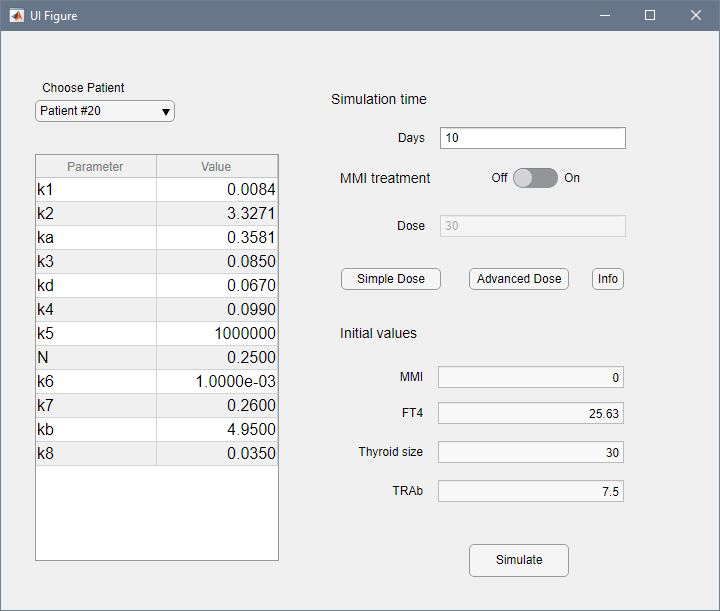
\includegraphics[width=1\textwidth]{specs/window1}
	\caption{Okno g��wne aplikacji.}\label{window1_img}
\end{figure}

\subsection{Wyb�r pacjenta}
W pierwszej cz�ci symulacji (Rys.~\ref{choose-patient_img}), u�ytkownik wybiera jednego z czterech analizowanych w pracy pacjent�w (Rys. \ref{patient-list_img}), dla kt�rego przeprowadzone zostan� symulacje. Parametry, charakterystyczne dla tego pacjenta zamieszczone s� w tabeli. Dodatkowych pacjent�w nale�y doda� z poziomu kodu.

\begin{figure}
	\centering
	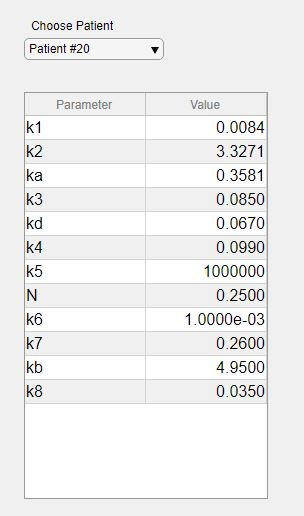
\includegraphics[width=0.4\textwidth]{specs/choose-patient}
	\caption{Wyb�r pacjenta.}\label{choose-patient_img}
\end{figure}

\begin{figure}
	\centering
	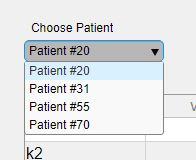
\includegraphics[width=0.4\textwidth]{specs/patient-list}
	\caption{Lista wyboru pacjenta.}\label{patient-list_img}
\end{figure}

\subsection{Wyb�r parametr�w symulacji}
Ta cz�� s�u�y do wyboru parametr�w symulacji (Rys. \ref{conf:simulation_img}): czasu, leczenia i dawki metimazolu. W pierszym polu u�ytkowanik wpisuje czas symulacji wyra�ony w dniach. U�ywaj�c w��cznika wybieramy leczenie lub jego brak. W��czenie terapii aktywuje pole dawki leku, w kt�rym wybieramy ilo�� metimazolu, jak� codziennie przyjmuje pacjent.

Terapie mog� by� bardzo skomplikowane, dlatego istnieje mo�liwo�� utworzenia schematu leczenia. Wystarczy wpisa� we wskazane pola kilka warto�ci po przecinku. Dla u�atwienia wprowadzania dawek, poni�ej umieszczono trzy dodatkowe przyciski (Rys. \ref{conf:simulation_img}). Pierwsze dwa: \textit{Simple Dose} i \textit{Advanced Dose}, automatycznie wpisuj� w pole \textit{Dose} domy�lne, przyk�adowe terapie. Trzeci przycisk \textit{Info} informuje, jak wype�nia� pola. Na rysunku (Rys. \ref{adv-treatment_img}) pokazano wprowadzenie przyk�adowego zaawansowanego schematu terapii.

\begin{figure}
	\centering
	\includegraphics[width=0.4\textwidth]{specs/simulation}
	\caption{Konfiguracja symulacji bez leczenia.}\label{conf:simulation_img}
\end{figure}

\begin{figure}
	\centering
	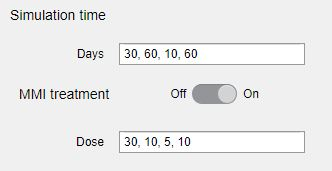
\includegraphics[width=0.4\textwidth]{specs/adv-treatment}
	\caption{Konfiguracja zaawansowanego leczenia.}\label{adv-treatment_img}
\end{figure}

\subsection{Warunki pocz�tkowe}

Wprowadzenie warunk�w pocz�tkowych odbywa automatycznie, po wyborze pacjenta (Rys. \ref{initial_img}). Poziom FT4, przeciwcia� i wielko�� kom�rek tarczycy ustalaj� si� po wyborze pacjenta, za� pole MMI ustawia si� po wybraniu dawki. 

\begin{figure}
	\centering
	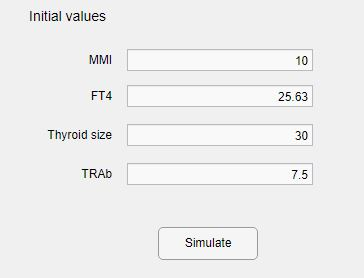
\includegraphics[width=0.4\textwidth]{specs/initial}
	\caption{Przyk�adowe warunki pocz�tkowe.}\label{initial_img}
\end{figure}

\subsection{Symulacja}
Naci�ni�cie przycisku \textit{Simulate}, rozpoczyna symulacj�. Przebieg symulacji potwierdza okno modalne z paskiem post�pu (Rys. \ref{progressbar_img}).
\begin{figure}
	\centering
	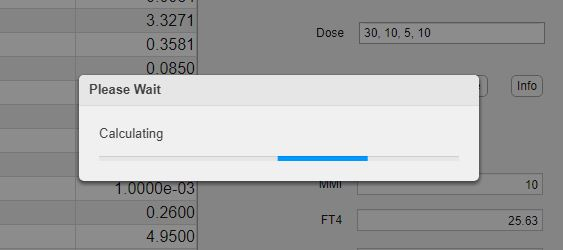
\includegraphics[width=0.6\textwidth]{specs/progressbar}
	\caption{Okno modalne oczekiwania na obliczenia.}\label{progressbar_img}
\end{figure}

\section{Okno wynik�w symulacji}
Okno wynik�w symulacji (Rys. \ref{window2_img}) pojawia si� po wykonaniu oblicze�. Po lewej stronie otrzymujemy przebiegi czasowe rozwi�za� modelu, za� po prawej wykresy zale�no�ci, kt�re mo�emy  ustali� wybieraj�c z paska kart odpowiednio odci�t� oraz rz�dn�. Nadrz�dna karta \textit{Details} wy�wietla tak�e szczeg�owe informacje o konfiguracji bie��cej symulacji.

\begin{figure}
	\centering
	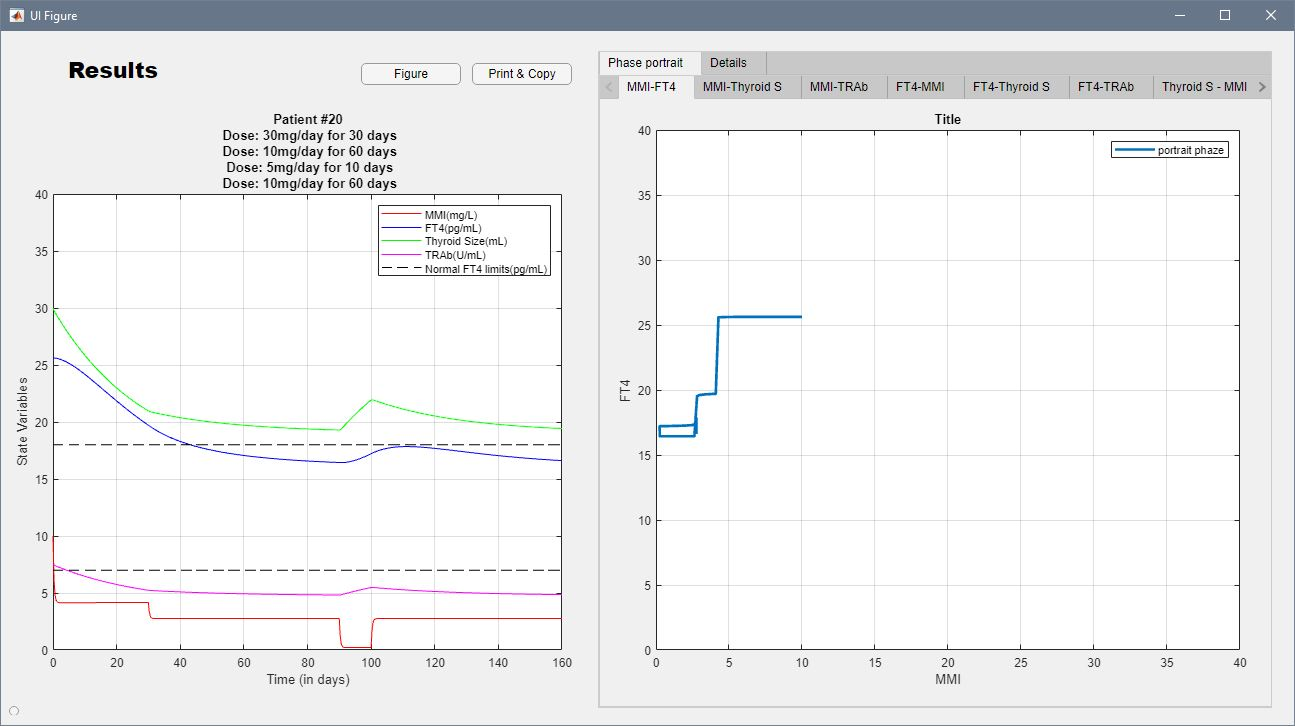
\includegraphics[width=1\textwidth]{specs/window2}
	\caption{Okno wynik�w symulacji.}\label{window2_img}
\end{figure}

\subsection{Graficzne przedstawienie wynik�w symulacji}
Przyk�adow� symulacj� leczenia pacjenta przedstawia rys. \ref{w2-simulation_img}. Wykres zawiera obszerny tytu� z istotnymi informacjami dotycz�cymi terapii pacjenta. Ka�da z funkcji stanu, jest narysowana odmiennym kolorem. Dla u�atwienia rozpoznania stadium choroby, przerywanymi poziomymi liniami zosta�y zaznaczone standardowe ilo�ci FT4 dla osoby zdrowej. Do wykresu do��czona jest legenda.

\begin{figure}
	\centering
	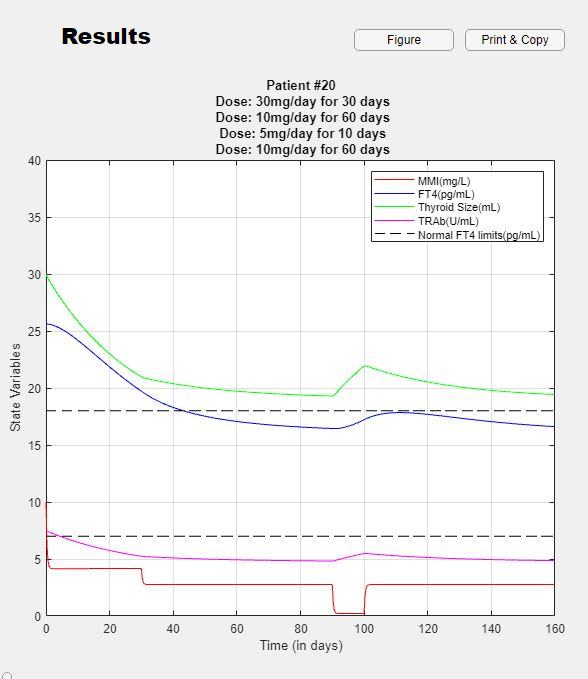
\includegraphics[width=0.8\textwidth]{specs/w2-simulation}
	\caption{Przyk�adowe przebiegi czasowe rozwi�za� modelu dla wskazanego w tytule schematu terapii.}\label{w2-simulation_img}
\end{figure}

Nad wykresem znajduj� si� dwa przyciski \textit{Figure} oraz \textit{Print~\&~Copy}. \textit{Figure} deleguje wykres do zaawansowanego narz�dzia edycji wykres�w (Rys. \ref{figure-gui_img}). Przycisk \textit{Print \& Figure} zapisuje wykres w katalogu programu, ze szczeg�ow� nazw� pliku oraz kopiuje go do schowka (Rys. \ref{img-path_img}).

\begin{figure}
	\centering
	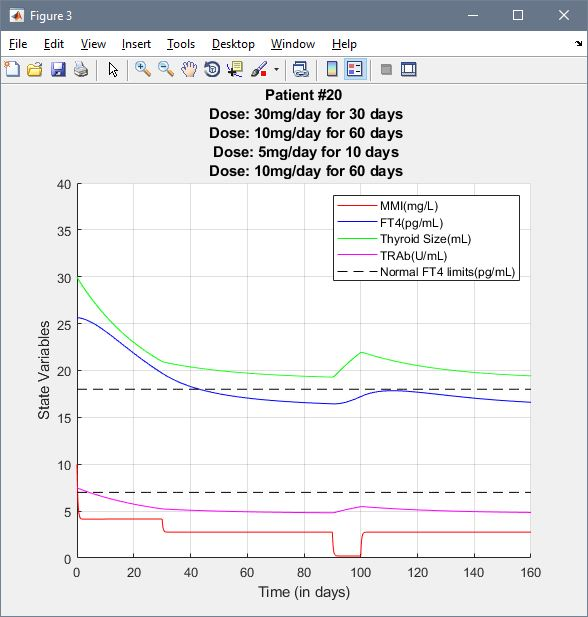
\includegraphics[width=0.8\textwidth]{specs/figure-gui}
	\caption{Narz�dzie edycji wykres�w.}\label{figure-gui_img}
\end{figure}

\begin{figure}
	\centering
	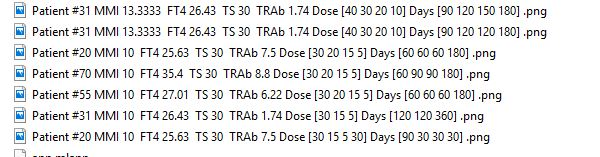
\includegraphics[width=0.8\textwidth]{specs/img-path}
	\caption{Zapisane w katalogu pliki wynik�w symulacji.}\label{img-path_img}
\end{figure}

\subsection{Portrety fazowe oraz szczeg�y symulacji}
Prawa cz�� okna wynik�w symulacji zawiera dwie zak�adki: \textit{Phase portrait} oraz \textit{Details}. Domy�lnie wy�wietlana jest zak�adka \textit{Phase portrait} (Rys.~\ref{portrait_img}), zawieraj�ca rzut portretu fazowego na okre�lon� przestrze� dwuwymiarow�. Dla funkcji okre�lonej w przestrzeni czterowymiarowej, takich rzut�w portret�w na przestrze� dwuwymiarow� jest 8.

\begin{figure}
	\centering
	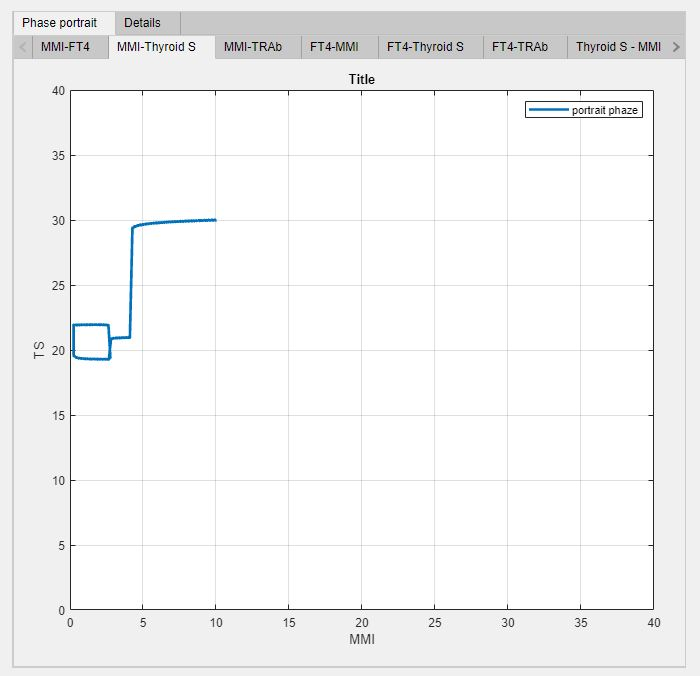
\includegraphics[width=0.8\textwidth]{specs/portrait}
	\caption{Przyk�adowy wykres zale�no�ci TS(MMI).}\label{portrait_img}
\end{figure}

Po naci�ni�ciu zak�adki \textit{Details}, otwiera si� cz�� informuj�ca u�ytkownika o szczeg�ach symulacji oraz o warto�ciach w�asnych Jacobianu w punkcie stacjonarnym (Rys.~\ref{details_img}), obliczonych dla wybranego pacjenta w przypadku braku leczenia.

\begin{figure}
	\centering
	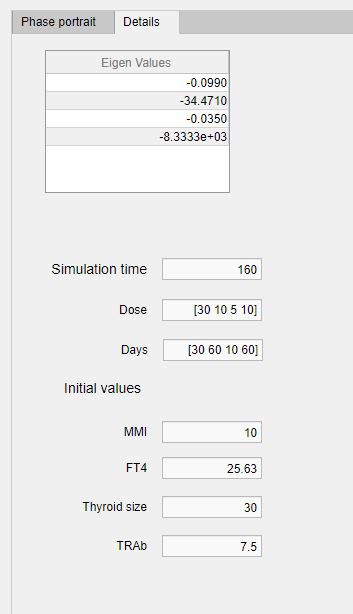
\includegraphics[width=0.5\textwidth]{specs/details}
	\caption{Szczeg�y symulacji oraz wyznaczone warto�ci w�asne Jacobianu w punkcie stacjonarnym dla przypadku braku terapi.}\label{details_img}	
\end{figure}

%%%%%%%%%%%%%%%%%%%%%%%%%%%%%%%%%%%%%%%%%%%%%%%%%%%%%%%%%%%%%%%%%%%%%%%%%%%%%%%%%%%%%%%%%%%%%%%%%%%%%%%%%%%%%%%%%%%%%%%%%%%%%%%%%%%%%%%%%%%%%%%%%%%%%%%%%%%%%%%%%%%%%%%
\chapter{Rezultaty} \label{sec:result}
%Zobrazowanie i om�wienie wynik�w otrzymywanych wskutek zastosowania danego urz�dzenia b�d� aplikacji. Badanie ewentualnych parametr�w (takich jak dok�adno��, czu�o��...), czy te� zachowania w szczeg�lnych sytuacjach. O ile to mo�liwe tabelaryzacja rezultat�w oraz ich statystyczna interpretacja. Ocena zachowania zaproponowanego rozwi�zania. Analiza mo�liwych przyczyn wyst�pienia b��d�w. 

W oparciu o program napisany przez autora pracy, symulowano r�ne scenariusze terapii pacjent�w. Do analizy modelu u�yto danych czterech pacjent�w (Rozdzia�. \ref{sec:dane}), zmagaj�cych si� z nadczynno�ci� tarczycy Gravesa�Basedowa. W tej cz�ci pracy zosta�y przedstawione symulacje leczenia chorych. 

\section{Wst�pne por�wnanie pacjent�w}

Na wykresie (Rys.~\ref{pacjenci_FT4_trab_img}) por�wnano analizowanych pacjent�w, ze wzgl�du na zmierzone warto�ci FT4 i TRAb. Badanie mia�o miejsce podczas pierwszej wizyty u lekarza. 

Na najsilniejsz� nadczynno�� tarczycy, zgodnie z poziomem hormonu FT4, cierpi pacjent numer 70. Potwierdza to r�wnie� najwy�szy poziom przeciwcia� TRAb w jego krwi. Poziom FT4 pozosta�ych pacjent�w jest zbli�ony. Pacjent numer 30 ma znacz�co ni�sz� warto�� przeciwcia�. Jego organizm mo�e by� bardzo czu�y na wyst�powanie przeciwcia� lub nadczynno�� jest spowodowana innym czynnikiem.

\begin{figure}
	\centering
	\includegraphics[width=1\textwidth]{excel/pacjenci_FT4_trab}
	\caption{Por�wnanie poziom�w FT4 i TRAb analizowanych pacjent�w.}\label{pacjenci_FT4_trab_img}
\end{figure}

\section{Pacjent numer 20}

\begin{figure}
	\centering
	\includegraphics[width=\size\textwidth]{wyniki/p20_no_dose_d10}
	\caption{Symulacja pacjenta nr 20 bez leczenia, trwaj�ca 10 dni.}\label{p20_no_dose_img}
\end{figure}

Na pocz�tku przeanalizowano stan pacjenta, bez podania leku. Poziom FT4 tego pacjenta wynosi� 25,63 pg/ml, co jest znacznie powy�ej normy (7-18 pg/ml). Dowodzi to faktu, i� pacjent ten cierpi na nadczynno�� tarczycy. Podczas symulacji trwaj�cej 10 dni, przebiegi czasowe rowi�za� modelu, czyli poziom MMI, FT4, rozmiar kom�rek gruczo�u i TRAb s� funkcjami sta�ymi, czyli nie zmieniaj� si� w czasie. Mo�na to zaobserwowa� na rysunku (Rys.~\ref{p20_no_dose_img}). Wraz z czasem d���cym do niesko�czono�ci sytuacja nie ulega zmianie. Wynika to z faktu, �e przy braku terapii, model jest asymptotycznie stabilny.

\begin{figure}
	\centering
	\includegraphics[width=\size\textwidth]{wyniki/p20_dose30_d1}
	\caption{Symulacja pacjenta nr 20, leczonego 30 mg leku, przez jeden dzie�.}\label{p20_dose30_d1_img}
\end{figure}

Po jednorazowym podaniu 30 mg MMI (Rys.~\ref{p20_dose30_d1_img}), lek zostaje ca�kowicie wydalony z organizmu w czasie jednego dnia. Ta dawka nie ma znacz�cego wp�ywu na funkcje tarczycy. 
 
\begin{figure}
	\centering
	\includegraphics[width=\size\textwidth]{wyniki/p20_dose30_d120}
	\caption{Symulacja pacjenta nr 20, leczonego 30 mg leku, przez 120 dni.}\label{p20_dose30_d120_img}
\end{figure}

Przy podawaniu 30 mg leku przez 120 dni, stan gospodarki hormonalnej tarczycy pacjenta, znacz�co si� zmieni� (Rys.~\ref{p20_dose30_d120_img}). Po oko�o 30 dniach, poziom FT4 pacjenta osi�gn�� graniczny stan dla osoby zdrowej. Kontynuowanie terapii przy tej samej dawce, skutkuje ci�g�ym obni�aniem si� poziomu tego hormonu i po 90 dniach osi�ga poziom �wiadcz�cy o niedoczynno�ci tarczycy.

\begin{figure}
	\centering
	\includegraphics[width=\size\textwidth]{wyniki/p20_dose30_d75_dose0_d45}
	\caption{Symulacja pacjenta nr 20 podczas leczenia i odstawienia leku.}\label{p20_dose30_d75_dose0_d45_img}
\end{figure}
  
Jak pokazano na rys.~\ref{p20_dose30_d75_dose0_d45_img} przy podawaniu dawki 30 mg przez 75 dni i nast�pnie odstawieniu leku, pacjent powr�ci� do stanu nadczynno�ci tarczycy. Trwa�o to oko�o 35 dni.  Taki scenariusz leczenia, okaza� si� nieskuteczny co oznacza, �e pacjent wymaga nast�pnej serii leczenia.

\begin{figure}
	\centering
	\includegraphics[width=\size\textwidth]{wyniki/p20_treatment}
	\caption{Symulacja dla pacjenta nr 20, przyk�adowa terapia, odstawienie i wznowienie terapii.}\label{p20_treatment_img}
\end{figure}

Rys. \ref{p20_treatment_img} przedstawia przyk�adow� terapi� dedykowan� dla pacjenta nr 20. Podczas leczenia dawk� 30 mg metimazolu przez 2 miesi�ce, st�enie FT4 pacjenta osi�gn�o g�rn� graniczn� warto�� po 27 dniach. Po 60 dniach st�enie to wynosi�o 12,3 pg/ml, dlatego postanowiono zwi�kszy� dawk� metizamolu do 40 mg dziennie. Graniczna warto�� zosta�a osi�gni�ta po 25 dniach, a st�enie FT4 pod koniec tego etapu terapii wynios�o 10,97 pg/ml. Nast�pnie zmniejszono dawk� do 20 pg/ml i dalej do 10 pg/ml. Po tym okresie trwaj�cym 4 miesi�ce, nale�y sprawdzi� czy choroba jest w stadium reemisji. Je�li tak, nale�y zacz�� kolejny etap leczenia, stosuj�c taki sam schemat dawkowania.

W artykue A. Prakash'a \cite{mmi}, opisane zosta�y r�ne metody leczenia choroby Gravesa. Niekt�re z bada� wskazuj�, �e du�e dawki metimazolu i kr�tka terapia zwi�kszaj� ryzyko wyst�pienia nawrot�w choroby. Optymalna d�ugo�� terapii powinna wynosi� 12-18 miesi�cy. Przy 18-miesi�cznej terapii, ryzyko nawrotu choroby to 37\%. 6-miesi�czna terapia wywo�a nawr�t u 58\% leczonych.

Stosuj�c si� do zalece� zawartych w artykule \cite{mmi}  opracowano terapi� dla pacjenta nr 20 (Rys.~\ref{p20_treatment1_img}). Podczas 12 miesi�cy co 2 miesi�ce dawka leku jest zmniejszana. Podawane s� dawki 30 mg MMI przez 2 miesi�ce, 20 mg przez 2 miesi�ce, 15 mg przez 2 miesi�ce i 5 mg przez 6 miesi�cy. W efekcie zaproponowanej terapii hormon FT4 pacjenta osi�ga poziom  FT4 cz�owieka zdrowego po 27 dniach leczenia.

\begin{figure}
	\centering
	\includegraphics[width=\size\textwidth]{wyniki/p20_treatment1}
	\caption{Symulacja dla pacjenta nr 20, sugerowana 12-miesi�czna terapia.}\label{p20_treatment1_img}
\end{figure}

\section{Pacjent numer 31}

Pacjent numer 31 jest odmiennym przypadkiem w odniesieniu do innych pacjent�w, gdy� poziom jego przeciwcia� jest niski przy podobnym st�eniu FT4. Symulacje wykaza�y (Rys. ~\ref{p31_treatment_img}), �e jest ma�o wra�liwy na leczenie metimazolem. Dla tego pacjenta, warto rozpatrywa� alternatywne metody leczenia. Sugerowane leczenie obejmuje wi�ksze dawki leku (Rys.~\ref{p31_treatment_img}). Trwa ono 18 miesi�cy, przy czym ostatnie 6 miesi�cy, pacjent pobiera dawk� 10 mg MMI. Podawane s� dawki 40 mg MMI przez pierwsze 3 miesi�ce, nast�pnie 30 mg przez 4 miesi�ce, 20 mg przez 5 miesi�cy i 10 mg przez ostatnie 6 miesi�cy.

\begin{figure}
	\centering
	\includegraphics[width=\size\textwidth]{wyniki/p31_treatment}
	\caption{Symulacja dla pacjenta nr 31, sugerowana 18-miesi�czna terapia.}\label{p31_treatment_img}
\end{figure}


\section{Pacjent numer 55}

\begin{figure}
	\centering
	\includegraphics[width=\size\textwidth]{wyniki/p55_treatment}
	\caption{Symulacja pacjenta nr 55, sugerowana 12-miesi�czna terapia.}\label{p55_treatment_img}
\end{figure}

Rys.~\ref{p55_treatment_img} przedstawia sugerowan� terapi� dla pacjenta numer 55. Zastosowano to samo leczenie, co w przypadku pacjenta nr 20 (Rys.~\ref{p20_treatment_img}). Podczas 12 miesi�cy co 2 miesi�ce dawka leku jest zmniejszana. Podawane s� dawki 30, 20, 15 i 5 mg MMI. Dawka podtrzymuj�ca leczenie wynosi 5 mg i jest podawana przez ostatnie 6 miesi�cy terapii. Pacjent osi�ga poziom FT4 odpowiadaj�cy g�rnej granicy FT4 dla osoby zdrowej po 29 dniach.

\section{Pacjent numer 70}

Pacjent nr 70 ma najwy�szy pocz�tkowy poziom hormonu FT4. Proponowana terapia trwa 14 miesi�cy (Rys.~\ref{p70_treatment_img}). Jako, �e jego poziom FT4 koreluje z wysokim poziomem przeciwcia� TRAb, chory dobrze reaguje na leczenie. Przez pierwsze 2 miesi�ce stosujemy dawk� 30 mg/dziennie, nast�pnie zmniejszamy dawk� do 20 i 15 mg, co 3 miesi�ce. Jako dawk� podtrzymuj�c� terapi� podajemy 5 mg leku przez 6 miesi�cy. Pacjent osi�ga poziom FT4 odpowiadaj�cy g�rnej granicy FT4 dla osoby zdrowej po 42 dniach.

\begin{figure}
	\centering
	\includegraphics[width=\size\textwidth]{wyniki/p70_treatment}
	\caption{Symulacja dla pacjenta nr 70, sugerowana 14-miesi�czna terapia.}\label{p70_treatment_img}
\end{figure}

\section{Por�wnanie zapotrzebowania na lek}

W niniejszym paragrafie przeanalizowano zapotrzebowanie na lek omawianych w pracy pacjent�w. Zsumowano ilo�� przyj�tego leku, podczas sugerowanego leczenia, przez okres pierwszych 360 dni. Dla pacjent�w nr 20, 31 jest to koniec terapii. Wyniki przedstawione zosta�y na rys.~\ref{pacjenci_mmi_img}. 3/4 pacjent�w przyjmie oko�o 5 g leku przez 12 miesi�cy. Pacjent numer 31 musi przyj�� 10 g leku przez 12 miesi�cy oraz b�dzie kontynuowa� leczenie przez kolejnych 6 miesi�cy.

\begin{figure}
	\centering
	\includegraphics[width=1\textwidth]{excel/pacjenci_mmi}
	\caption{Por�wnanie zapotrzebowania na lek pacjent�w.}\label{pacjenci_mmi_img}
\end{figure}

%%%%%%%%%%%%%%%%%%%%%%%%%%%%%%%%%%%%%%%%%%%%%%%%%%%%%%%%%%%%%%%%%%%%%%%%%%%%%%%%%%%%%%%%%%%%%%%%%%%%%%%%%%%%%%%%%%%%%%%%%%%%%%%%%%%%%%%%%%%%%%%%%%%%%%%%%%%%%%%%%%%%%%%
\chapter{Podsumowanie}

\section{Wnioski}
\begin{itemize}
\item Model pozwala symulowa� terapie, jednak wyznaczenie parametr�w $k_5$, $k_6$ polega na minimalizacji b��du �redniokwadratowego wzgl�dem poprzednich terapii pacjenta \ref{sec:params}. W zwi�zku z tym, niemo�liwe jest stosowanie symulacji, dla pacjent�w podczas ich pierwszej wizyty, a ilo�� wcze�niejszych terapii zwi�ksza dok�adno�� modelu.

\item Poniewa� parametry $k_5$ i $k_6$ s� symulowane, modelu nie mo�na zastosowa� we wspomaganiu terapii pacjenta, gdy� indywidualno�� ich wyznaczania jest czasoch�onna i korzysta z danych konkretnego pacjenta z poprzednich terapii. Jednak, je�li wyznaczymy te parametry, model powinien znacz�co podnie�� efektywno�� terapii, poprzez dobranie optymalnej �cie�ki leczenia, dawek oraz pozwoli� efektywnie zaplanowa� kolejne wizyty, zmniejszaj�c tym samym ilo�� bada� oraz orzeka� o reemisji lub wyleczeniu z wi�kszym prawdopodobie�stwem \ref{sec:result}.

\item W por�wnaniu do modelu skonstruowanego przez Langensteinam \cite{old-model} model zastosowany w pracy Pandiyan \cite{graves1}, kt�ry bazuje na pracy poprzednika, pozwala obserwowa� przebieg czasowy metimazolu w krwi. Wprowadza to wiele niedom�wie� oraz symulacje, kt�re dotycz� r�nych d�ugo�ci terapii nie s� zbie�ne. Nieintuicyjnym lub niemo�liwym jest te�  wyznaczenie prawdopodobie�stwa reemisji, dla symulowanej terapii.

\item Symulacja przebieg�w czasowych nie jest czynnikiem, kt�ry bezpo�rednio wp�ywa na efektywno�� terapii pacjenta. Wa�niejszym jest wyznaczenie prawdopodobie�stwa reemisji wzgl�dem terapii. W leczeniu choroby Gravesa, dob�r w�a�ciwych dawek i oscylacja mi�dzy prawid�owymi poziomami FT4 mo�e pozytywnie wp�ywa� na ca�kowite wyleczenie, jednak hipoteza ta musi zosta� przebadana w przysz�o�ci.

\item Symulacja przebieg�w czasowych pozwala na w�a�ciwy dob�r dawek leczenia, sprawiaj�c, �e gospodarka hormonalna uk�adu tarczycowego b�dzie funkcjonowa�a tak, jak u cz�owieka zdrowego \ref{sec:result}. Znacz�co zmniejsza si� ryzyko przedawkowania leku, kt�re mo�e doprowadzi� do niedoczynno�ci tarczycy lub zwi�kszenia efekt�w ubocznych przyjmowania metimazolu. Wp�ywa na zdrowie i komfort �ycia pacjenta.

\item Optymalizacja kodu, poprzez stosowanie w�a�ciwych metod, mo�e znacz�co zwi�kszy� wydajno�� aplikacji i zmniejszy� zu�ycie zasob�w. Zastosowanie przeci��enia metody, pozwoli�o zmniejszy� zapotrzebowanie na pami�� RAM czterokrotnie i znacz�co skr�ci�o obliczenia \ref{sec:functions}. Pozwoli�o to na wykonanie wi�kszej liczby symulacji. 
\end{itemize}
%Nawi�zanie do celu pracy oraz postawionych za�o�e�. Pr�ba oceny realizacji celu, poprzez weryfikacj� otrzymanych rezultat�w. Analiza dostrze�onych problem�w, b��dnego, nieoczekiwanego dzia�ania, ewentualnych problem�w napotkanych podczas realizacji. W przypadku niewyczerpania tematu, a tak�e wspomnianego niepo��danego zachowania urz�dzenia/aplikacji sugestie ich eliminacji wymienione jako plany na przysz�o��.\footnote{Kr�tkie! 1-2 strony.}
%
%Wst�p wraz z podsumowaniem winny stanowi� swego rodzaju klamr�, a nawet ca�o�� w takim rozumieniu, �e przeczytanie wy��cznie tych dw�ch rozdzia��w t�umaczy� powinno rozwa�any problem wraz z efektami otrzymanymi w efekcie prac, stanowi�cymi jego rozwi�zanie, bez wnikania w spos�b ich otrzymania (to zawiera cz�� �rodkowa).


%\appendix  % <--- zaczynaj� si� dodatki; jak nazywa si� rozdzia� -> szuka� appendixname powy�ej
%\chapter{Obliczenia}
W dodatku umieszczamy opis ewentualnych znanych algorytm�w, z kt�rych korzystamy proponuj�c w�asn� metodologi�, opisan� w rozdziale~\ref{Chapter_Metodologia}. Wykaz pozycji literaturowych tworzymy w oddzielnym pliku \texttt{Praca.bib}. Chc�c si� odwo�a� w tek�cie do wybranej pozycji bibliograficznej korzystamy z komendy \texttt{cite}. Efekt jej u�ycia dla kilku pozycji jednocze�nie to~\cite{Tadeusiewicz,Malina,Nieniewski_Morfologia}.

%%%%%%%%%%%%%%%%%%%%%%%%%%%%%%%%%%%%%%%%%%%%%%%%%%%%%%%%%%%%%%%%%%%%%%%%%%%%%%%%%%%%%%%%%%%%%%%%%%%%%%%%%%%%%%%%%%%%%%%%%%%%%%%%%%%%%%%%%%%%%%%%%%%%%%%%%%%%%%%%%%%%%%%
\chapter{Dodatek B}
Podstawowe kwestie techniczne dotycz�ce wzor�w, rysunk�w, tabel poni�ej.

Wzory tworzymy w �rodowisku \texttt{equation}. Chc�c odwo�a� si� do wybranego wzoru gdzie� w tek�cie nale�y nada� mu stosown�, niepowtarzaln� i jednoznaczn� etykiet�, po ty by m�c np. napisa� zdanie: ze wzoru~\ref{Wzor_Dodawanie} wynika \ldots
\begin{equation}\label{Wzor_Dodawanie}
	c = a + b
\end{equation}

Wzory z�o�one, charakteryzuj�ce si� przypisaniem warto�ci zmiennej w pewnych okoliczno�ciach tworzymy przy u�yciu otoczenia \texttt{eqnarray}. Odwo�anie do wzoru jak wcze�niej. 
\begin{eqnarray}\label{equ_progowanie}
    BW & = & \left \{
    \begin{array}{ll}
      1, & I(x,y) \geq T \\
      0, & I(x,y) < T\\
    \end{array}
    \right.,
\end{eqnarray}

% \subsection{Usuwanie numeracji przy r�wnaniach}

Numeracj� r�wna� mo�na tymczasowo (w~danej linijce) wy��czy� poprzez u�ycie $\backslash{}nonumber$
\begin{eqnarray}
	a_i = a_{i-1}+a_{i-2}\nonumber \\ % w tej linijce nie ma numeru
              +a_{i-3}
\end{eqnarray}


\section{Wstawianie rysunk�w}
Rysunki umieszczamy w otoczeniu \texttt{figure}, centruj�c je w poziomie komend� \texttt{centering}. Rozmiary rysunku ustalamy w komendzie \texttt{includegraphics} dobieraj�c wielko�� wzgl�dem rozmiaru strony lub bezwzgl�dnie np. w cm. Ponadto najpierw zapowiadamy pojawienie si� rysunku w tek�cie (czyli np. Na rysunku (Rys~\ref{Rysunek_LogoIB}) pracy, a dopiero p�niej wstawiamy sam rysunek. Dodatkowo sterowa� mo�emy umiejscowieniem rysunku na stronie dzi�ki parametrom \texttt{[!htb]} okre�laj�cym miejsce. Odpowiednio s� to: \texttt{here}, \texttt{top}, \texttt{bottom}. 
\begin{figure}[!htb]
	\centering
	
\includegraphics[width=.35\textwidth]{logo/logoRIB}
	\caption{Logo Wydzia�u In�ynierii Biomedycznej.}\label{Rysunek_LogoIB}
\end{figure}

Do��czaj�c rysunki nie trzeba podawa� rozszerzenia (wr�cz jest to odradzane). Je�li rysunki znajduj� si� w~katalogu \emph{rysunki}, nie trzeba r�wnie� podawa� �cie�ki do nich.

\section{Wstawianie tabelek}
Analogicznie post�pujemy z tabelkami, z t� r�nic� �e tworzymy j� w otoczeniu \texttt{table}. W nim natomiast sam� tabel� definiujemy albo w �rodowisku \texttt{tabular}, albo \texttt{tabularx}. Podobnie z odwo�aniami w tek�cie: najpierw odwo�anie w Tab.~\ref{Tabelka_Tabela}, a dopiero p�niej sama tabela.
\begin{table}[!htb]
	\centering
	\topcaption{Opis nad tabelk�.}\label{Tabelka_Tabela}
	\begin{tabular}{|c|c|c|c|} \hline \hline 
		Kolumna 1 & Kolumna 2 & Kolumna 3 & Kolumna 4 \\ \hline
		Wiersz 1 & & & \\ \hline
		Wiersz 2 & & & \\ \hline
		Wiersz 3 & & & \\ \hline
		& & & \\ \hline
		& & & \\ \hline
	\end{tabular}
\end{table}

%%%%%%%%%%%%%%%%%%%%%%%%%%%%%%%%%%%%%%%%%%%%%%%%%%%%%%%%%%%%%%%%%%%%%%%%%%%%%%%%%%%%%%%%%%%%%%%%%%%%%%%%%%%%%%%%%%%%%%%%%%%%%%%%%%%%%%%%%%%%%%%%%%%%%%%%%%%%%%%%%%%%%%%
\chapter{Kwestie edytorskie}
Zbi�r zasad pomocnych przy redagowaniu tekstu pracy wystarczaj�co szczeg�owo przedstawia ksi��ka~\cite{Chwalowski}.

Uwaga! Pisz�c prac� nale�y zwr�ci� uwag� na nast�puj�ce kwestie:
\begin{enumerate}
	\item Prace piszemy w formie bezosobowej.
	\item Unikamy okre�le� potocznych, spolszcze� funkcjonuj�cych codziennej mowie itp.
	\item Pos�uguj�c si� znanymi nam (a nie czytelnikowi) has�ami (r�wnie� skr�tami, akronimami) najpierw je definiujemy i~t�umaczymy, a~dopiero p�niej traktujemy za znane.
	\item Podpisy pod rysunkami lub nad tabelami traktujemy jak zdania, a wi�c powinny stanowi� sp�jn� ca�o�� oraz powinny zosta� zako�czone kropk�.
	\item Podobnie wypunktowania (po dwukropku kolejne punkty pisane ma�ymi literami, oddzielane przecinkami, ostatni zako�czony kropk� o ile ko�czy zdanie).
	\item Do ka�dego rysunku, tabeli, pozycji bibliograficznej musi istnie� odwo�anie w tek�cie pracy, przy czym do pierwszych dw�ch musi si� ono pojawi� zanim umie�cimy rysunek/tabel�.
\end{enumerate}


\clearpage \addcontentsline{toc}{chapter}{\bibname}
\bibliography{Praca}


\end{document}
